%% History:
% Pavel Tvrdik (26.12.2004)
%  + initial version for PhD Report
%
% Daniel Sykora (27.01.2005)
%
% Michal Valenta (3.12.2008)
% rada zmen ve formatovani (diky M. Duškovi, J. Holubovi a J. Žďárkovi)
% sjednoceni zdrojoveho kodu pro anglickou, ceskou, bakalarskou a diplomovou praci

% One-page layout: (proof-)reading on display
%%%% \documentclass[11pt,oneside,a4paper]{book}
% Two-page layout: final printing
\documentclass[11pt,twoside,a4paper]{book}   
%=-=-=-=-=-=-=-=-=-=-=-=--=%
% The user of this template may find useful to have an alternative to these 
% officially suggested packages:
\usepackage[czech, english]{babel}
\usepackage[T1]{fontenc} % pouzije EC fonty 
% pripadne pisete-li cesky, pak lze zkusit take:
% \usepackage[OT1]{fontenc} 
\usepackage[utf8]{inputenc}
%=-=-=-=-=-=-=-=-=-=-=-=--=%
% In case of problems with PDF fonts, one may try to uncomment this line:
%\usepackage{lmodern}
%=-=-=-=-=-=-=-=-=-=-=-=--=%
%=-=-=-=-=-=-=-=-=-=-=-=--=%
% Depending on your particular TeX distribution and version of conversion tools 
% (dvips/dvipdf/ps2pdf), some (advanced | desperate) users may prefer to use 
% different settings.
% Please uncomment the following style and use your CSLaTeX (cslatex/pdfcslatex) 
% to process your work. Note however, this file is in UTF-8 and a conversion to 
% your native encoding may be required. Some settings below depend on babel 
% macros and should also be modified. See \selectlanguage \iflanguage.
%\usepackage{czech}  %%%%%\usepackage[T1]{czech} %%%%[IL2] [T1] [OT1]
%=-=-=-=-=-=-=-=-=-=-=-=--=%

%%%%%%%%%%%%%%%%%%%%%%%%%%%%%%%%%%%%%%%
% Styles required in your work follow %
%%%%%%%%%%%%%%%%%%%%%%%%%%%%%%%%%%%%%%%
\usepackage{graphicx}
\usepackage{float}
\usepackage{amssymb}
%\usepackage{indentfirst} %1. odstavec jako v cestine.

\usepackage{k336_thesis_macros} % specialni makra pro formatovani DP a BP
 % muzete si vytvorit i sva vlastni v souboru k336_thesis_macros.sty
 % najdete  radu jednoduchych definic, ktere zde ani nejsou pouzity
 % napriklad: 
 % \newcommand{\bfig}{\begin{figure}\begin{center}}
 % \newcommand{\efig}{\end{center}\end{figure}}
 % umoznuje pouzit prikaz \bfig namisto \begin{figure}\begin{center} atd.


%%%%%%%%%%%%%%%%%%%%%%%%%%%%%%%%%%%%%
% Zvolte jednu z moznosti 
% Choose one of the following options
%%%%%%%%%%%%%%%%%%%%%%%%%%%%%%%%%%%%%
% \newcommand\TypeOfWork{Diplomová práce} \typeout{Diplomova prace}
% \newcommand\TypeOfWork{Master's Thesis}   \typeout{Master's Thesis} 
\newcommand\TypeOfWork{Bakalářská práce}  \typeout{Bakalarska prace}
% \newcommand\TypeOfWork{Bachelor's Project}  \typeout{Bachelor's Project}


%%%%%%%%%%%%%%%%%%%%%%%%%%%%%%%%%%%%%
% Zvolte jednu z moznosti 
% Choose one of the following options
%%%%%%%%%%%%%%%%%%%%%%%%%%%%%%%%%%%%%
% nabidky jsou z: http://www.fel.cvut.cz/cz/education/bk/prehled.html

%\newcommand\StudProgram{Elektrotechnika a informatika, dobíhající, Bakalářský}
%\newcommand\StudProgram{Elektrotechnika a informatika, dobíhající, Magisterský}
% \newcommand\StudProgram{Elektrotechnika a informatika, strukturovaný, Bakalářský}
% \newcommand\StudProgram{Elektrotechnika a informatika, strukturovaný, Navazující magisterský}
\newcommand\StudProgram{Softwarové technologie a management, Bakalářský}
% English study:
% \newcommand\StudProgram{Electrical Engineering and Information Technology}  % bachelor programe
% \newcommand\StudProgram{Electrical Engineering and Information Technology}  %master program


%%%%%%%%%%%%%%%%%%%%%%%%%%%%%%%%%%%%%
% Zvolte jednu z moznosti 
% Choose one of the following options
%%%%%%%%%%%%%%%%%%%%%%%%%%%%%%%%%%%%%
% nabidky jsou z: http://www.fel.cvut.cz/cz/education/bk/prehled.html

%\newcommand\StudBranch{Výpočetní technika}   % pro program EaI bak. (dobihajici i strukt.)
%\newcommand\StudBranch{Výpočetní technika}   % pro prgoram EaI mag. (dobihajici i strukt.)
\newcommand\StudBranch{Softwarové inženýrství}            %pro STM
%\newcommand\StudBranch{Web a multimedia}                  % pro STM
%\newcommand\StudBranch{Computer Engineering}              % bachelor programe
%\newcommand\StudBranch{Computer Science and Engineering}  % master programe


%%%%%%%%%%%%%%%%%%%%%%%%%%%%%%%%%%%%%%%%%%%%
% Vyplnte nazev prace, autora a vedouciho
% Set up Work Title, Author and Supervisor
%%%%%%%%%%%%%%%%%%%%%%%%%%%%%%%%%%%%%%%%%%%%

\newcommand\WorkTitle{Systém pro výpočet softwarových metrik}
\newcommand\FirstandFamilyName{Martin Ovesný}
\newcommand\Supervisor{Ing. Ladislav Vágner, Ph.D.}


% Pouzijete-li pdflatex, tak je prijemne, kdyz bude mit vase prace
% funkcni odkazy i v pdf formatu
\usepackage[
pdftitle={\WorkTitle},
pdfauthor={\FirstandFamilyName},
bookmarks=true,
colorlinks=true,
breaklinks=true,
urlcolor=red,
citecolor=blue,
linkcolor=blue,
unicode=true,
]
{hyperref}

\begin{document}

%%%%%%%%%%%%%%%%%%%%%%%%%%%%%%%%%%%%%
% Zvolte jednu z moznosti 
% Choose one of the following options
%%%%%%%%%%%%%%%%%%%%%%%%%%%%%%%%%%%%%
\selectlanguage{czech}
%\selectlanguage{english} 

% prikaz \typeout vypise vyse uvedena nastaveni v prikazovem okne
% pro pohodlne ladeni prace


\iflanguage{czech}{
	 \typeout{************************************************}
	 \typeout{Zvoleny jazyk: cestina}
	 \typeout{Typ prace: \TypeOfWork}
	 \typeout{Studijni program: \StudProgram}
	 \typeout{Obor: \StudBranch}
	 \typeout{Jmeno: \FirstandFamilyName}
	 \typeout{Nazev prace: \WorkTitle}
	 \typeout{Vedouci prace: \Supervisor}
	 \typeout{***************************************************}
	 \newcommand\Department{Katedra počítačů}
	 \newcommand\Faculty{Fakulta elektrotechnická}
	 \newcommand\University{České vysoké učení technické v~Praze}
	 \newcommand\labelSupervisor{Vedoucí práce}
	 \newcommand\labelStudProgram{Studijní program}
	 \newcommand\labelStudBranch{Obor}
}{
	 \typeout{************************************************}
	 \typeout{Language: english}
	 \typeout{Type of Work: \TypeOfWork}
	 \typeout{Study Program: \StudProgram}
	 \typeout{Study Branch: \StudBranch}
	 \typeout{Author: \FirstandFamilyName}
	 \typeout{Title: \WorkTitle}
	 \typeout{Supervisor: \Supervisor}
	 \typeout{***************************************************}
	 \newcommand\Department{Department of Computer Science and Engineering}
	 \newcommand\Faculty{Faculty of Electrical Engineering}
	 \newcommand\University{Czech Technical University in Prague}
	 \newcommand\labelSupervisor{Supervisor}
	 \newcommand\labelStudProgram{Study Programme} 
	 \newcommand\labelStudBranch{Field of Study}
}




%%%%%%%%%%%%%%%%%%%%%%%%%%    Titulni stranka / Title page 

\coverpagestarts

%%%%%%%%%%%%%%%%%%%%%%%%%%%    Podekovani / Acknowledgements 

\acknowledgements
\noindent
Rád bych na tomto místě poděkoval Ing. Ladislavu Vágnerovi, Ph.D. za poskytnutí velice zajímavého tématu a za odborné vedení mé bakalářské práce.



%%%%%%%%%%%%%%%%%%%%%%%%%%%   Prohlaseni / Declaration 

\declaration{V~Praze dne \today} %26.\,5.\,2010
%\declaration{In Kořenovice nad Bečvárkou on May 15, 2008}


%%%%%%%%%%%%%%%%%%%%%%%%%%%%    Abstract 
 
\abstractpage

\noindent
This thesis is focused on software source quality measures by software metrics evaluation. There are discussed size-oriented metrics,
complexity measures as their association with white-box testing and object-oriented metrics for design flaws detection.

\noindent
Outcome from the work is software metrics evaluation system that is easy to extend by modules. Results of system's computation are compared to
some of the existing software discussed in the text.

% Prace v cestine musi krome abstraktu v anglictine obsahovat i
% abstrakt v cestine.
\vglue60mm

\noindent{\Huge \textbf{Abstrakt}}
\vskip 2.75\baselineskip

\noindent
Práce je zaměřena na problematiku vyhodnocování kvality zdrojových kódů pomocí softwarových metrik. V~textu jsou popsány
softwarové metriky orientované na velikost kódu, metriky zabývající se složitostí kódu a její souvislostí s~white-box testováním
a objektově orientované metriky vyhodnocující správný objektový návrh.

\noindent
Výsledkem práce je systém pro výpočet softwarových metrik, který je snadno rozšiřitelný formou modulů, a porovnání
jeho činnosti s~některými programy uvedenými v~textu.

%%%%%%%%%%%%%%%%%%%%%%%%%%%%%%%%  Obsah / Table of Contents 

\tableofcontents


%%%%%%%%%%%%%%%%%%%%%%%%%%%%%%%  Seznam obrazku / List of Figures 

\listoffigures


%%%%%%%%%%%%%%%%%%%%%%%%%%%%%%%  Seznam tabulek / List of Tables

%\listoftables


%**************************************************************

\mainbodystarts
% horizontalní mezera mezi dvema odstavci
%\parskip=5pt
%11.12.2008 parskip + tolerance
\normalfont
\parskip=0.2\baselineskip plus 0.2\baselineskip minus 0.1\baselineskip

% Odsazeni prvniho radku odstavce resi class book (neaplikuje se na prvni 
% odstavce kapitol, sekci, podsekci atd.) Viz usepackage{indentfirst}.
% Chcete-li selektivne zamezit odsazeni 1. radku nektereho odstavce,
% pouzijte prikaz \noindent.

%**************************************************************

% Pro snadnejsi praci s vetsimi texty je rozumne tyto rozdelit
% do samostatnych souboru nejlepe dle kapitol a tyto potom vkladat
% pomoci prikazu \include{jmeno_souboru.tex} nebo \include{jmeno_souboru}.
% Napr.:
% \include{1_uvod}
% \include{2_teorie}
% atd...

%*****************************************************************************
\chapter{Úvod}

\section{Zařazení výpočtu softwarových metrik do procesu vývoje software}
S~tím, jak v~softwarovém inženýrství doba pokročila, se staly požadavky na čas dodání a nasazení
softwaru kritickými faktory. Proto je nutné vývoj co nejlépe zoptimalizovat, aby nedocházelo ke zbytečným ztrátám zisku.
Proces vývoje software skládající se z~analýzy, návrhu, implementace, testování a údržby je již pevně zavedený ve velkém
množství softwarových společností. Vyhodnocení kvality (kontrola jakosti) zdrojových kódů pomocí softwarových metrik se dá
v~tomto procesu zařadit ke dvojici implementace-testování. Právě s~testováním mají softwarové metriky úzkou souvislost \cite{CCN,NPATH,MCCABEWHATSON96}.
Respektováním jejich výsledků mohou vývojáři zajistit, aby nebyly jednotlivé části software zbytečně složité,
což udrží i složitost testování nižší. Tím se zároveň program stává průhledným a snižuje se pravděpodobnost, že se v~testech
opomene kontrola některých možných průběhů testovaného programu. Pokud by pak v~této části vznikla chyba, bylo by velice obtížné
a drahé ji dohledávat, protože výsledky testů by ukazovaly, že je vše v~pořádku.

Fakt, že zařazení kontroly jakosti do procesu vývoje software nese dobré výsledky, potvrzuje například to, že ho do svého
vývojového procesu zařadila i organizace NASA\cite{NASA} nebo společnosti jako Microsoft, Electronic Arts, Intel, Siemens, Hewlett-Packard
a další \cite{NDepend}.

\section{Cíl práce}
\label{sec:Cil}
Cílem práce je vytvoření systému pro výpočet softwarových metrik, jenž bude moduly snadno rozšiřitelný.
Tyto moduly budou umožnovat rozšíření o~další vstupní jazyky a o~výpočet dalších softwarových metrik nebo jiný způsob vyhodnocení kvality
zdrojových kódů (např. kontrola dodržování kódovacích konvencí - odsazování, pojmenování, apod.).
Výsledný program by měl být vhodný pro automatické vyhodnocení kvality kódu studentských prací (domácí úkoly,
semestrální práce). Program na vstupu dostane zdrojový kód nebo skupinu zdrojových kódů a na výstupu
zapíše výsledky do XML souboru.

K~tomu, aby bylo možné systém realizovat, je potřeba nejdříve zjistit jaké softwarové metriky existují, a zpracovat
jejich přesné definice. Podle nich bude systém kvalitu kódu vyhodnocovat. Jedná se o~metriky, které se dají
vypočítat pouze z~předložených zdrojových kódů. Systém tudíž nebude mít k~dispozici statistiky z~jiných projektů,
čímž jsou vyloučeny metriky pro časové a finanční odhady. Nicméně výsledný systém by mělo být možné rozšířit o~moduly,
které takové odhady počítat umí.

\section{Struktura práce}
V~kapitole \ref{sec:KvalitaKodu} tohoto textu je představeno několik metod vyhodnocení kvality zdrojových kódů.
Jsou v~ní podrobně popsány některé nejznámější a nejpoužívanější softwarové metriky.
Následuje kapitola \ref{sec:ExistujiciSW} obsahující výčet již existujících programů,
které metriky počítají. Jedná se o~nástroje, jenž patří mezi nejrozšířenější, nejlepší a
nebo mají nějakou zvláštní funkcionalitu, díky které stojí za zmínku.

Kapitola \ref{sec:Navrh} se zabývá návrhem systému pro výpočet softwarových metrik definovaného v~kapitole \ref{sec:Cil}.
Kromě popisu architektury a jeho jednotlivých částí, popisuje i použití nově vznikajícího standardu Abstract Syntax Tree Metamodel,
který vytvořila Object Management Group.

V~kapitole \ref{sec:Realizace} je popsán způsob implementace některých důležitých částí realizovaného systému. Popisována je
zejména realizace frontendu pro jazyk C++. Frontend byl vytvořen pokročilými postupy v~dvojici nástrojů Flex a Bison. Následující
kapitola \ref{sec:Testovani} pak diskutuje výstupy metrik, které realizovaný systém implementuje. Některé z~nich jsou porovnány s~výsledky,
kterých bylo dosaženo softwarem popsaným v~kapitole \ref{sec:ExistujiciSW}.

Na přiloženém CD se pak nachází implementace samotného systému pro výpočet softwarových metrik.


%*****************************************************************************
\chapter{Analýza}

\section{Vyhodnocení kvality zdrojových kódů}
\label{sec:KvalitaKodu}
Kvalita zdrojových kódů může být vyhodnocována buď manuálně, nebo automatizovaně. Manuální vyhodnocení spočívá v~tom,
že programátor, který zkoumaný zrojový kód nezná, si ho pročítá a snaží se ho pochopit. Výsledkem je pak report,
ve kterém je uvedeno například, kde je kód zbytečně složitý nebo je upozorněno na nedodržování domluvených konvencí, apod.
Hlavní nevýhodou tohoto způsobu je, že čas, který programátor stráví nad prováděním revize, by mohl daleko lépe vyplnit
nějakou tvůrčí činností. Zde nastupuje vyhodnocení automatické, které se snaží udělat práci za člověka.
Automatické vyhodnocení se dá rozdělit do dvou kategorií: statická analýza \cite{static_analysis} a dynamická analýza \cite{dynamic_analysis}.

\paragraph{Dynamická analýza} se používá například k~zjišťování, zda software správně pracuje s~přidělenými prostředky
(uvolňuje paměť, zavírá file descriptory, apod.) nebo ke kontrole běhu vláken (např. nalezení deadlocku), apod.
Tato analýza je prováděna tím způsobem, že je program spuštěn a za běhu jsou sbírány informace o~jeho průběhu.
Některé nástroje pro dynamickou analýzu (např. Valgrind \cite{Valgrind}) pouští testovaný proces přes svůj vlastní virtuální procesor.
Jiné (např. Mudflap \cite{Mudflap}, jenž je součástí projektu GCC) zase linkují své knihovny do zkoumaného programu,
aby měly kontrolu nad některými funkcemi pro práci s~\mbox{dynamickou} pamětí, apod. Dynamická analýza je tedy kvůli spouštění
závislá na testovacích datech, které ovlivňují chování testovaného programu. Je tudíž nezbytné, aby byla tato data správně zvolena,
jinak by se neotestovaly všechny případy toho, jak může program v~závislosti na vstupech proběhnout.

\paragraph{Statická analýza}, naopak od té dynamické, nespouští analyzovaný program a výpočty se provádí přímo na
jeho zdrojových kódech nebo, v~některých případech (např. nástroj Vil\cite{Vil}), na přeloženém kódu. Typicky se statická analýza
používá na výpočet softwarových metrik, upozornění na některé nevhodné konstrukce, ve kterých může být ukrytá
chyba (tzv. lint\cite{lint} nebo bug patterns\cite{bug_patterns}), ke kontrole dodržování předepsaných konvencí, apod.
Výsledky statické analýzy pak slouží například k~rychlejšímu ladění aplikací, upozornění na chyby v~návrhu, které
nebyly dosud odhaleny nebo, v~neposlední řadě, ke statistikám, které mohou projektovým manažerům poskytnout orientační
informace o~kvalitě a \mbox{výkonnosti} jednotlivých programátorů, což může mít vliv na časové a finanční odhady budoucích projektů.

\subparagraph{Softwarová metrika} je definována\cite{SciTech04} jako pravidlo pro vyčíslení nějaké vlastnosti určité části zkoumaného softwaru.
Metriky se snaží vývojářům prozradit hlavně to, zda je software správně navržen a zda je jeho kód přehledný, což jsou dva
faktory, které jdou spolu ruku v~ruce. Softwarové metriky mají význam v~celém vývojovém procesu (analýza, návrh, implementace,
testování, údržba) a souvisejí tedy i s~dalšími disciplínami softwarového inženýrství.

Použití softwatových metrik však nekončí u~zdrojového kódu. Existují i metriky, které jsou přímo určené na
časové odhady a odhady finančních prostředků pro budoucí projekty (např. Function Point Analisis \cite{FPA} nebo metrika COCOMO \cite{COCOMO}).
Tyto metriky ale používají empirické metody, pro které jsou potřeba statistiky z~předchozích projektů. Navíc takové
odhady se provádějí před započetím implementace, tudíž je není možné počítat ze zdrojových kódů (ještě neexistují)
jako ty, kterými se tento text zabývá.

\subsection{Softwarové metriky orientované na velikost zdrojového kódu}
Tato skupina metrik patří mezi nejjednodušeji vypočítatelné, nejpoužívanější a také nejstarší.
Požívaly se na hodnocení výkonosti programátotů už v~dobách, kdy se vůbec o~nějakých  metrikách nevědělo.
Dnes mají poněkud jiný význam, protože výkonost se tímto měřit nedá, jelikož dnešní programátor má na starosti
daleko více než jen psaní zdrojového kódu (návrh, testování, dokumentace, apod.).

Softwarové metriky orientované na velikost zdrojového kódu mají nevýhodu v~tom, že jsou velmi závislé na zvoleném
programovacím jazyku, tudíž je potřeba toto vzít v~úvahu při vyhodnocování jejich výsledků. Dále je problém i v~tom,
že změřené hodnoty mohou být odlišné u~různých programátorů, pokud nejsou striktně stanovena pravidla na to,
jak má být kód formátován, protože každý má svůj styl odsazování, závorkování, atd.

\subsubsection{File Size}
Velikost souboru je nejzákladnější softwarovou metrikou, která udává počet bajtů v~souboru.

\subsubsection{Source Lines Of Code}
Vyskytuje se v~několika variantách, protože počet řádků, který metrika udává, se dá podat různými způsoby.
Souhrně se všechny varianty nazývají Source Lines Of Code (SLOC).

Základní variantou je Lines Of Code (LOC) \cite{SLOC}, která udává počet všech rádků v~souboru. Vzhledem k~tomu, že hodnota
nemusí být zcela vypovídající kvůli k~tomu, že v~zdrojovém kódu mohou být prázdné řádky či komentáře, přichází
na řadu druhá varianta, nazývaná Logical Lines Of Code (LLOC) \cite{LLOC}. LLOC
udává počet řádků v~souboru, do kterých se nezapočítávají zmíněné prázdné řádky a komentáře. Řádka se počítá jako komentář
v~momentě, kdy na ní je pouze komentář. Pokud by na ní byl nějaký kus kódu, který by byl na konci řádku okomentován,
pak se řádek počítá jako kód, nikoli jako komentář.

Ovšem i LLOC může obsahovat kód, který není relevantní (například direktivy preprocesoru v~C/C++).

Při vyhodnocení této metriky je tedy vždy potřeba definovat, co se do ní započítává, protože když budeme
očekávat LLOC hodnotu a místo ní se vrátí LOC, může být rozdíl i řádový.

Tyto metriky se nepoužívají pouze ke zjištění, kolik řádků má celý soubor. Stejně dobře je lze využít i pro výpočet toho,
jak obsáhlé jsou jednotlivé funkce programu nebo klidně i celý systém dohromady. Případně průměrné a maximální hodnoty,
odchylky od průměru, apod.

U~všech zmíněných variant SLOC metriky platí, že při vysokých hodnotách na výstupu, je vysoká i pravděpodobnost,
že je program špatně navržen a měl by být rozdělen do více modulů (funkcí, tříd, souborů, ...).

\subsubsection{Lines Lengths}
Metrika zjišťuje kolik znaků je na jednotlivých řádcích kódu a vypočítá maximální a průměrnou délku ve funkci, či souboru.

\subsubsection{Comments density}
\label{sec:MCOMM}
Jedná se o~procentuální vyjádření toho, jaká část z~kódu je zabrána komentáři. Variant výpočtu je opět několik.
Jednou z~možností je například hrubý výpočet pomocí SLOC:
$$COMM\% = (LOC - LLOC) / LOC$$
Výpočet se dá upřesnit \cite{MCOMM} například ještě zohledněním prázdných rádků nebo dokonce vyhodnocením toho,
které komentáře jsou významné a které naopak nenesou žádnou informaci:
$$MCOMM\% = MCOMM / LLOC$$
MCOMM je zkratka pro Meaningful Comments, címž se myslí počet komentářů (nemusí se jednat pouze
o~celořádkové komentáře), které obsahují alespoň jedno písmeno. Nepočítají se tedy prázdné komentáře
nebo komentáře používané na zpřehledňování, které obsahují například samé pomlčky, apod.

\subsection{Softwarové metriky orientované na složitost programu}
Tato kategorie metrik dohání nedostatky té předchozí hlavně v~tom, že výsledky těchto metrik
opravdu vypovídají o~tom, jak je program složitý, protože nepočítají pouze počet řádků, ale analyzují
i to, co se na nich nachází. Další výhodou oproti předchozí skupině metrik je fakt, že
nezáleží na zvoleném jazyku a na stylu zápisu programatora, protože se počítá přímo se složitostí
jednotlivých operací, ze kterých se program sestává (příkazy, výrazy).

Tyto metriky také přímo souvisí s~testováním \cite{MCCABEWHATSON96}, protože jejich výsledky se dají interpretovat i jako míra toho,
jak složité je analyzované části systému testovat (viz. CCN a NPATH dále v~textu).

\subsubsection{McCabe’s Cyclomatic Complexity}
\label{sec:CCN}
Cyklomatická složitost byla prezentována v~roce 1976 matematikem Thomasem J. McCabem, podle něhož bývá často nazývána.
Metrika ve své podstatě udává počet všech cest, kterými lze program projít. K~tomu, aby bylo možné cyklomatickou složitost
definovat, je potřeba nejdříve zavést pojem Control Flow Graph.

\paragraph{Definice:}\cite{NPATH,CCN} Control Flow Graph (CFG) je orientovaný graf ($V$, $E$, $V_{entry}$, $V_{exit}$), kde
\begin{itemize}
 \item $V$ je množina uzlů grafu, kde každý uzel reprezentuje blok kódu (sekvenci příkazů, které program nevětví) nebo nějakou větvící konstrukci (if, while, ...)
 \item $E$ je množina hran grafu, kde každá hrana, reprezentuje větev programu, kterou může program probíhat (Control Flow Path)
 \item $V_{entry}$ je prvek množiny $V$, který reprezentuje unikátní vstupní uzel
 \item $V_{exit}$ je prvek množiny $V$, který reprezentuje unikátní výstupní uzel
\end{itemize}
Dále platí, že z~uzlu $V_{entry}$ existuje orientované spojení do všech ostatních uzlů grafu a zároveň ze všech těchto uzlů grafu
musí existovat orientované spojení do uzlu $V_{exit}$.
\begin{flushright}$\blacksquare$\end{flushright}

\paragraph{Definice:}\cite{CCN} Cyklomatická složitost $V(G)$ grafu $G$ obsahujícího $n$ vrcholů, $e$ hran a $p$ komponent je
$$V(G) = e - n + 2p$$
\begin{flushright}$\blacksquare$\end{flushright}

Cyklomatická složitost $V(G)$ se často označuje zkratkou CCN (Cyclomatic Complexity Number).

V~následujících větách a tvrzeních se navíc uvažuje hrana orientovaná z~$V_{exit}$ do $V_{entry}$, aby v~každém CFG existoval alespoň jeden cyklus
(viz. obrázek \ref{fig:ccn_vcg}).

\begin{figure}[H]
\begin{center}
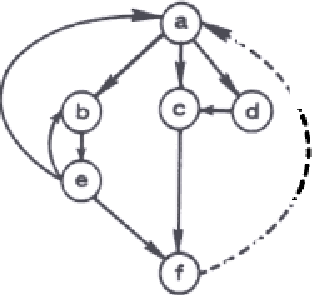
\includegraphics[width=4cm]{figures/ccn_cfg.pdf}
\caption{Control Flow Graph: uzly $a = V_{entry}$ a $f = V_{exit}$ jsou spojeny čárkovanou hranou, která se do CFG přidává navíc, aby byla v~grafu vždy alespoň jeden cyklus.}
\label{fig:ccn_vcg}
\end{center}
\end{figure}

\paragraph{Věta:} V~silně souvislém grafu $G$ je cyklomatická složitost rovna maximálnímu počtu \mbox{lineárně} nezávislých cyklů.
\begin{flushright}$\blacksquare$\end{flushright}

Každý cyklus v~CFG tvoří jeden prvek báze lineárního prostoru všech cest v~grafu $G$, takže je možné pomocí jejich lineárních
kombinací sestavit libovolný podgraf. Hodnost této báze je hledané $V(G)$.

Podle předchozích tvrzení by se mohlo zdát, že v~definici $V(G)$ je zbytečná proměnná $p$. Není tomu tak, protože $p$ reprezentuje
jednotlivé funkční jednotky programu, takže CCN lze vypočítat pro jednotlivé funkce ($v(G)$) stejně tak, jako pro moduly nebo dokonce celý systém ($V(G)$).
Například na následujícím obrázku je hlavní funkce M, která volá funkce A~a B. Každá funkce je jedna komponenta.

\begin{figure}[H]
\begin{center}
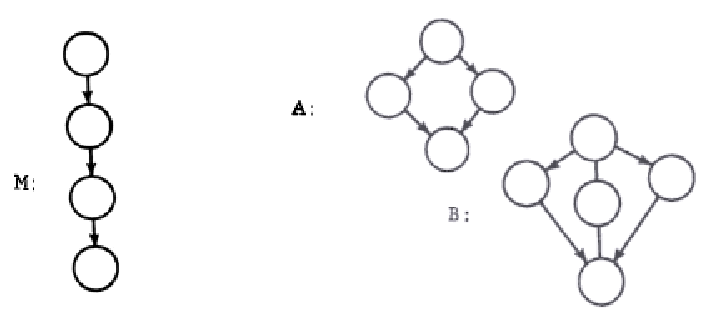
\includegraphics[width=7cm]{figures/ccn_functions.pdf}
\caption{CFG pro více funkčních jednotek. Hlavní funkce $M$ volá funkce $A$ a $B$.}
\label{fig:ccn_functions}
\end{center}
\end{figure}

Složitost takového systému je pak $V(G) = v(A \cup B \cup C) = e - n + 2p = 13 - 13 + 2 * 3 = 6$.

\paragraph{Tvrzení:}
Hodnota $V(G)$ grafu $G$ obsahující komponenty $G_1, ..., G_n$ dá vypočítat jako
$$V(G) = \sum_{i=1}^n{v(G_i)}$$

\paragraph{Důkaz:}
$$V(G) = e - n + 2p = \sum_{i=1}^p{e_i} - \sum_{i=1}^p{n_i} + 2p = \sum_{i=1}^p{(e_i - n_i + 2)} = \sum_{i=1}^p{v(G_i)}$$
\begin{flushright}$\blacksquare$\end{flushright}

Pokud tedy známe CCN dílčích funkcí, pak lze složitost systému spočítat jejich pouhým sečtením:
$V(G) = v(A \cup B \cup C) = v(A) + v(B) + v(C) = 1 + 2 + 3 = 6$.

V~praxi se ovšem program nepřevádí do grafu, nýbrž se využije následujícího zjednodušení (platí pouze pro jazyky pro strukturované
programování - pro jazyky nestrukturovaného programování, jako je například assembler, je postup popsán v~\cite{CCN}).

Nechť $\theta$ je počet funkcí a $\pi$ je počet predikátů\footnote{Predikát = rozhodovací konstrukce programovacího jazyka (if, while, ...)},
pak počet hran $e$ v~grafu $G$ je
$$e = 1 + \theta + 3\pi$$

Dále každý predikát $\pi$ je v~grafu $G$ znázorněn jedním uzlem, který se větví do dvou dalších uzlů (nezáleží na tom, zda jde také o~predikát, nebo ne)
a každá funkce $\theta$ má jeden vstupní a jeden výstupní uzel, takže počet uzlů $n$ v~grafu $G$ je
$$n = \theta + 2\pi + 2$$

Pro $p = 1$ platí
$$v(G) = e - n + 2p = (1 + \theta + 3\pi) - (\theta + 2\pi + 2) + 2 = \pi + 1,$$
tedy $v(G)$ je rovno počtu predikátů (větvení) plus jedna.

\begin{figure}[H]
\begin{center}
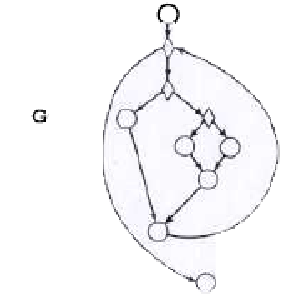
\includegraphics[width=4cm]{figures/ccn_simplify_example.pdf}
\caption{Graf $G$ obsahující $e$ hran a $n$ uzlů. Kosočtverce značí predikáty.}
\label{fig:ccn_simplify_example}
\end{center}
\end{figure}


\paragraph{Rozšíření CCN na CCN2}
Už sám McCabe navrhnul \cite{CCN}, že by bylo žádoucí započítávat do složitosti i složené výrazy v~podmínkách, protože například zápis
\begin{verbatim} if(c1 && c2) ... \end{verbatim}
je potřeba uvažovat dekomponovaný na
\begin{verbatim} if(c1) if(c2) ... ,\end{verbatim}
ve kterém jsou zřetelné dva predikáty, nikoli jeden, jako je tomu v~prvním zápisu. Proto se zavádí CCN2, kde se tento fakt
bere v~úvahu a při výpočtu se k~počtu predikátů navíc přičítá počet operátorů \&\& a ||.

\paragraph{Dalších rozšíření} McCabovy složitosti je hodně, protože tato metrika byla často diskutována a jiní autoři
(např. Knots, McClure, Myers, Nejmeh, Piwowarski, ...) \cite{CCN_extra} cítili, že
by ji šlo dále modifikovat, aby bylo dosaženo lepších výsledků než podle její původní definice.

\paragraph{Výsledná hodnota CCN} má souvislost s~white-box testováním \cite{CCN}, protože vyjadřuje \textbf{minimální} počet všech různých konfigurací
vstupních hodnot pro testovanou funkci potřebný pro to, aby bylo splněno code coverage kritérium\footnote{Code coverage kritérium je jedním
z~pravidel úspěšného testování \cite{CodeCoverage}. Podmínkou jeho splnění je, že všechny podmíněné výrazy a podvýrazy budou vyhodnoceny jako \textit{true}
i jako \textit{false}, všechny větve programu budou provedeny, všechny příkazy v~programu budou provedeny a všechny funkce v~programu budou zavolány.}.

Obecně je doporučováno udržovat CCN ve funkci do hodnoty 10, v~případě použití \mbox{varianty} CCN2 do hodnoty 20. Tyto hodnoty jsou sice rozumné,
ale ne všemohoucí, protože se do CCN nebere v~úvahu například zanořování rozhodovacích konstrukcí (je daleko složitější ladit a testovat
několik vnořených cyklů než stejný počet cyklů jdoucích po sobě). Stejně tak se nezapočítávají váhy jednotlivých konstrukcí,
takže podmínky mají stejnou váhu jako cykly. Dalším takovým příkladem, kdy CCN pokulhává, může být velký \textit{switch} s~mnoha \textit{case} větvemi.
Konkrétně tento případ se uvádí jako tolerovaný a vysoká hodnota CCN se pak promíjí.

\subsubsection{Nejmeh's NPATH Complexity}
\label{sec:NPATH}
Brian A. Nejmeh zavádí svoji NPATH složitost kvůli nedostatkům McCabovy složitosti hlavně v~tom, že nebere
v~úvahu zanořování rozhodovacích konstrukcí. I~když tato metrika vychází z~teorie grafů podobně jako McCabova
složitost, tak ji Nejmeh definoval \cite{NPATH} výčtem algoritmů výpočtu na jednotlivých syntaktických konstrukcích jazyka C.

\paragraph{Příkaz if:}
\begin{verbatim}
if(<expr>)
  <if-body>
\end{verbatim}
$$NP(if) = NP(<expr>) + NP(<if-body>) + 1$$

\paragraph{Příkaz if-else:}
\begin{verbatim}
if(<expr>)
  <if-body>
else
  <else-body>
\end{verbatim}
$$NP(if-else) = NP(<expr>) + NP(<if-body>) + NP(<else-body>)$$

\paragraph{Příkaz while:}
\begin{verbatim}
while(<expr>)
  <while-body>
\end{verbatim}
$$NP(while) = NP(<expr>) + NP(<while-body>) + 1$$

\paragraph{Příkaz do-while:}
\begin{verbatim}
do
  <do-body>
while(<expr>)
\end{verbatim}
$$NP(do-while) = NP(<expr>) + NP(<do-body>) + 1$$

\paragraph{Příkaz for:}
\begin{verbatim}
for(<expr1>; <expr2>; <expr3>)
  <for-body>
\end{verbatim}
$$NP(for) = NP(<expr1>) + NP(<expr2>) + NP(<expr3>) + NP(<for-body>) + 1$$

\paragraph{Příkaz switch:}
\begin{verbatim}
switch(<expr>)
{
  <case1>
  ...
  <casen>
  <default>
}
\end{verbatim}
$$NP(switch) = NP(<expr>) + NP(<default>) + \sum_{i=1}^{n}{<case_i>}$$
Pokud je <$case_i$> prázdný (neobsahuje žádný příkaz), pak je jeho $NP = 1$.

\paragraph{Výraz s~ternárním operátorem:}
\begin{verbatim}
<expr1> ? <expr2> : <expr3>
\end{verbatim}
$$NP(?:) = NP(<expr1>) + NP(<expr2>) + NP(<expr3>) + 2$$
Dvojka na konci vzorce se přičítá kvůli tomu, že bez ní by šlo pouze o~součet složitostí jednotlivých výrazů. Díky ní se do $NP(?:)$ započítá
i fakt, že ternární operátor vytváří další větev (hranu v~CFG) stejně jako například \textit{if}.

\paragraph{Příkazy goto a continue} se do $NP$ vůbec nezapočítávají.

\paragraph{Příkaz break} má hodnotu $NP(break) = 1$.

\paragraph{Příkaz return:}
\begin{verbatim}
return <expr>
\end{verbatim}
$$NP(return) = NP(<expr>)$$

\paragraph{Výrazy} se započítávají pouze tehdy, když obsahují operátory logického součinu nebo logického součtu.
\begin{verbatim}
<expr1> op1 <expr2> op2 ... op(N-1) <exprN>
\end{verbatim}
$$NP(vyraz) = ({pocet\ operatoru\ \&\&}) + ({pocet\ operatoru\ ||})$$

\paragraph{Ostatní příkazy} nevětvící tok programu, včetně volání funkcí, mají $NP = 1$.

\paragraph{Funkce:}
$$NPATH = \prod_{i=1}^{i=N}{NP(prikaz_i)},$$
kde $N$ je počet příkazů ve funkci.

\paragraph{Výsledná hodnota NPATH} má, stejně jako CCN, význam v~testování \cite{NPATH}, protože hodnota $NPATH$ je rovna \textbf{maximálnímu} počtu
všech různých konfigurací vstupních hodnot pro testovanou funkci potřebných k~tomu, aby bylo splněno code coverage kritérium.

\subsubsection{McClure's Complexity}
Carma L. McClure představila další možný způsob \cite{MC} jak určit složitost programu.
$$Complexity = C + V,$$
kde $C$ je počet podmínek a $V$ je počet unikátních proměnných, které v~těchto podmínkách figurují.

\subsubsection{Decision Density}
\label{sec:DECDENS}
Metrika vyjadřuje, jak je daná funkce opticky přehledná a srozumitelná. Počítá se jako poměr rozhodovacích konstrukcí vůči celkovému počtu operací
\cite{PMComplexity}, zjednodušeně:
$$DECDENS = CCN / LLOC$$

\subsubsection{Henry's and Kafura's (HK) Information Flow Metrics}
\label{sec:HK}
S. Henry a D. Kafura přišli s~myšlenkou, že složitost zkoumaného systému je tím vyšší, čím víc jeho částí je vájemně provázaných.

Metoda, kterou tuto složitost určují je dána vztahem \cite{HKMYW}:
$$Complexity = [procedure-length] * [fan-in * fan-out]^2,$$
kde $fan-in$ je informace, která do funkce přišla (in) z~venčí, tedy počet funkcí, které zkoumaná funkce volá, zatímco $fan-out$
je informace, která odešla (out), tedy počet volání zkoumané funkce jinými funkcemi. $Procedure-length$ je délka funkce a nemusí
jít pouze o~její fyzickou velikost (SLOC), ale i o~výstup jakékoli relevantní metriky, například CCN, NPATH, apod.
Autoři tuto proměnnou schválně blíže nespecifikovali.

\subsubsection{Data Structure Metrics}
Jedná se o~skupinu metrik, které se snaží vyčíst složitost programu z~toho, s~jakým objemem dat nebo s~jakým typem dat pracuje.
Typicky se počítá počet proměnných deklarovaných ve funkci a počet proměnných, které funkce deklaruje jako parametry.

Lze uvažovat i \uv{život} proměnných, tzn. kde byla jaká proměnná použita poprvé a kde naposledy. Hlavní idea takové analýzy je v~tom,
že se metrika snaží zjistit s~kolika proměnnými programátor v~dané jednotce pracuje a kolik jich tedy musí brát
v~úvahu při testování, či úpravách jednotky.

\subsubsection{Halstead's Metrics}
Maurice Howard Halstead představil v~roce 1977 další způsob, jak vyčíslit složitost programu. Jedná se o~celou skupinu několika fomulí,
a proto se v~některých zdrojích tato metrika označuje jako Halstead's Software Science \cite{SWQMetrics}.

Halstead předpokládá, že každý program lze přepsat na seznam tokenů a každý z~nich lze klasifikovat buď jako operátor, nebo jako operand.
Abeceda programu $n$ je definována jako
$$n = n_1 + n_2,$$
kde $n_1$ je počet všech unikátních operátorů (např. pro $*$, $*$, $+$ je $n_1 = 2$) a $n_2$ je počet všech unikátních operandů.
Dalším atributem pro výpočet je délka programu, která je definována jako
$$N = N_1 + N_2,$$
kde $N_1$ je počet všech operátorů (např. pro $*$, $*$, $+$ je $n_1 = 3$) a $N_2$ je počet všech operandů.

Z~výše definovaných proměnných se dá spočítat \uv{objem} programu jako
$$V = N*\log_2{(n)}$$

Halsteadovy výzkumy prokázály, že hodnota $V$ se mění lineárně v~porovnání se SLOC.

Konečně pro výpočet toho, jak je složité programu porozumět ($D$ = Difficulty), slouží následující vztah:
$$D = (n_1 / 2) * (N_2 / n_2)$$

Tato metrika může sloužit nejen k~výpočtu složitosti existujícího programu, ale dokonce i k~odhadu složitosti programu,
který se teprve chystá a z~toho se dá také odhadnout, jaké usilí ($E$ = Effort - množství času, programátorů, finančních prostředků)
bude potřeba k~napsání takového programu \cite{MILLS88}.
$$E = D * V$$

Jako pomoc pro odhad délky zatím neimplementovaného programu může posloužit další vztah, se kterým Halstead přišel.
Jedná se o~způsob, jak odhadnout délku programu $N'$ pomocí abecedy programu $n_1, n_2$, která je snáze odhadnutelná.
$$N' = n_1 * \log_2{(n_1)} + n_2 * \log_2{(n_2)}$$

Odhad délky může sloužit i k~určení, jak \uv{přímočaře} je program následně implementován ($L$ = program Level). Uvažujme například následující dva způsoby,
jak vypočítat mocninu $x^y$ v~C++ ($x$ a $y$ jsou celá čísla a $y \geq 0$):
\begin{verbatim}
1. double res = pow(x, y);
2. double res = 1; for(int i = 0; i < y; i++) res *= x;
\end{verbatim}

Myšlenka spočívá v~tom, že se porovná předem odhadnutá délka programu proti jeho reálné délce, když už byl implementován. 
K~tomu slouží vzorec
$$L = N' / N$$
Díky hodnotě $L$ se dají korigovat budoucí odhady.

\paragraph{Hodnocení Halsteadovy metriky} není dobré \cite{MARCO97,CMM}, protože se na ni po její publikaci snesla vlna kritiky.
Metrika má velkou nevýhodu v~tom, že výsledné hodnoty jsou samy o~sobě naprosto nevýřečné, protože nikde není definováno,
jak jaký jazyk přeložit na sekvenci operandů a operátorů, takže to záleží vždy na implementaci stejně tak, jako na vstupním
jazyku (Pascal, C++, Assembler, ...).

\subsection{Softwarové metriky orientované na objektový návrh}
Objektově orientované metriky (tzv. strukturální analýza) se snaží zkoumat, zda třída,
či skupina tříd, dodržují pravidla správného návrhu, jako je například ortogonální návrh \cite{Pragmatik}
nebo Demeterovo pravidlo \cite{Pragmatik}. Analýza je prováděna podle deklarací jednotlivých tříd,
tzn. například podle dědičnosti, metod nebo členských proměnných a jejich vlastností.
Vzhledem k~tomu, že jeden takovýto samotný atribut (metrika), jako je například počet
potomků, nic moc o~hierarchii tříd v~systému nevypovídá, jsou tyto metriky charakteristické tím, že jejich výstupem
není jedna hodnota, jako tomu bylo u~předchozích, ale jedná se většinou o~celou skupinu hodnot, které se
snaží vytvořit určitý obraz o~zkoumaném systému. Nicméně existují i vyjímky, jako jsou například
{kohezní metriky}\footnote{Skupina kohezních metrik vychází z~metriky LCOM (Lack of Cohesion of Methods) \ref{sec:LCOM}.},
které samy o~sobě charakterizují zkoumanou třídu poměrně dobře.

\subsubsection{Chidamber-Kemerer (CK) metrics}
V~roce 1994 vydali Shyan R. Chidamber a Chris F. Kemerer článek \cite{CK94}, kde prezentovali svou sotfwarovou metriku pro
objektově orientovaný návrh známou také pod názvem \mbox{MOOSE} (Metrics for Object-Oriented Software Engineering) \cite{LKaMOODextra},
která se skládá z~následujících atributů:

\paragraph{Weight Methods per Class (WMC):} Mějme třídu $C$, která má metody $M_1, ..., M_n$ a $c_1, ..., c_n$
jsou složitosti jednotlivých metod. Potom platí:
$$WMC=\sum_{i=1}^{n}{c_i}$$
WMC je tedy suma složitostí všech metod, definovaných v~rámci dané třídy. Složitost $c_i$ není schválně nijak
blíže určena, takže je možné za ni dosadit výstup nějaké jiné metriky, jako například cyklomatickou složitost
nebo počet řádků. Stejně tak je možné za ni dosadit konstantu a pak WMC vyjadřuje počet metod definovaných
v~rámci třídy.

\subparagraph{Důsledky WMC}
\begin{enumerate}
\item Počet metod a jejich složitosti, které jsou do WMC zahrnuty předpovídají, kolik práce a času bude potřeba k~vývoji a udržování třídy.
\item Čím více má třída metod, tím větší vliv má třída na své potenciální potomky.
\item Třídy s~velkým počtem metod bývají dosti specifické, což může být na úkor \mbox{znovupoužití}.
\end{enumerate}


\paragraph{Depth of Inharitance Tree (DIT)} je definována jako maximální vzdálenost ve stromu dědičnosti od zkoumané třídy ke kořenu.
Vzdálenost je maximální, protože v~některých jazycích (např. C++), existuje možnost vícenásobné dědičnosti.
DIT vyjadřuje míru ovlivnitelnosti zkoumané třídy svými předchůdci, ze kterých třída dědí.

\subparagraph{Důsledky DIT}
\begin{enumerate}
\item Čím hlouběji je třída ve stromu dědičnosti, tím větší počet metod dědí, což dělá třídu složitejší na porozumění.
\item Stromy s~velkou hloubkou bývají návrhově složitější, protože zahrnují velký počet tříd a metod.
\item Čím hlouběji v~hierarchii se třída nachází, tím větší je možnost znovupoužití děděných metod.
\end{enumerate}

\paragraph{Number Of Children (NOC)} je počet přímých potomků zkoumané třídy a vyjadřuje,
kolik jiných tříd bude dědit její metody.

\subparagraph{Důsledky NOC}
\begin{enumerate}
\item Čím více potomků zkoumaná třída má, tím větší je míra jejího znovupoužití.
\item Čím více potomků zkoumaná třída má, tím vyšší je pravděpodobnost, že je špatně navržena. Hierarchie tříd by měla být spíše hlubší než širší.
\item Pokud má třída hodně potomků, je možné, že bude složitější testování jak jí samotné, tak i jejích potomků.
\end{enumerate}

\paragraph{Coupling Between Object classes (CBO)} je číslo udávající počet jiných tříd, se kterými je zkoumaná třída spárovaná.
Třídy jsou spárované tehdy, když jedna třída používá metody nebo členské proměnné definované v~nějaké jiné třídě.
CBO tedy vyjadřuje míru závislosti zkoumané třídy na jiných třídách.

\subparagraph{Důsledky CBO}
\begin{enumerate}
\item Přehnaná závislot mezi třídami odporuje správnému modulárnímu návrhu a značně snižuje možnost znovupoužitelnosti závislé třídy.
\item Čím více je třída závislá na jiných, tím je složitější její udržování, protože je daleko víc citlivá na změny v~jiných místech systému.
\item Čím vyšší je závislost mezi třídami, tím nutnější bude jejich důkladné testování.
\end{enumerate}

\paragraph{Response For a Class (RFC)} je definována jako počet prvků množiny $RS$ (Response Set),
tedy
$$RFC = |RS|.$$
$RS$ je definováno jako sjednocení množiny metod zkoumané třídy s~množinami
všech metod, které jsou volány z~metod třídy, tedy
$$RS = \{M\} \cup_{all}\ _i\ \{R_i\},$$
kde $\{R_i\}$
je množina metod volaných metodou $M_i$ a $\{M\}$ je množina metod definovaných ve zkoumané třídě.
$RS$ třídy je tedy množina metod, které mohou být vykonány při potenciálním volání nějaké metody
zkoumané třídy. Vzhledem k~tomu, že jsou do této množiny zahrnuty i metody definované mimo třídu,
dá se RFC interpretovat jako množství komunikace mezi zkoumanou třídou a jinýmy částmi systému,
ve kterém se třída nachází.

\subparagraph{Důsledky RFC}
\begin{enumerate}
\item Vysoká hodnota RFC může být známkou toho, že je třída složitá na porozumění, s~čímž souvisí i její složitější testování.
\end{enumerate}

\paragraph{Lack of Cohesion of Methods (LCOM)}
\label{sec:LCOM}
\subparagraph{Definice:} Mějme třídu $C$, která má $n$ metod $M_1, ..., M_n$.
Dále nechť $\{I_j\}$ je množina {instančních proměnných}\footnote{Instanční proměnná je členská
proměnná třídy, kterou mezi sebou jednotlivé její instance nesdílejí, což znamená, že pro každou instanci třídy
existuje jedna kopie takové proměnné.} použitých metodou $M_i$. Těchto množin je celkem $n$: $\{I_1\}, ..., \{I_n\}$,
tedy jedna pro každou z~metod. Nechť $P = \{(I_i, I_j)|I_i \cap I_j = \emptyset\}$ a
$Q = \{(I_i, I_j)|I_i \cap I_j \neq \emptyset\}$. Pokud jsou všechny množiny $\{I_1\}, ..., \{I_n\}$ prázdné,
pak i $P = \emptyset$.
$$LCOM = |P| - |Q|,\ pokud\ |P| > |Q|$$
$$LCOM = \emptyset,\ pokud\ |P| \leq |Q|$$
\begin{flushright}$\blacksquare$\end{flushright}

Hodnota LCOM tedy vyjadřuje počet párů metod, které nepoužívají stejné instanční proměnné mínus
počet párů metod, které používají stejné instanční proměnné. Výsledek lze interpretovat jako
míru podobnosti mezi metodami uvnitř třídy $C$ nebo dokonce jako sourodost (kohezi) třídy.
Čím je hodnota LCOM vyšší, tím je vyšší i podobnost metod a tedy i sourodost třídy.

\subparagraph{Důsledky LCOM}
\begin{enumerate}
\item Sourodost třídy je žádoucí, protože zvyšuje úroveň zapouzdření.
\item Nedostatečná sourodost je známkou toho, že by třída měla být rozdělena na několik menších tříd.
\item Jakákoli nesourodost metod může odhalit vážné chyby při návrhu tříd.
\item Nízká sourodost třídy zvyšuje její složitost, což zvyšuje i pravděpodobnost výskytu chyb.
\end{enumerate}

\subparagraph{Vylepšení LCOM:} po představení CK metriky byla následně několika dalšími autory diskutována a vylepšována
a zejména díky atributu LCOM začala vznikat celá skupina metrik zabývajících se sourodostí metod třídy
(tzv. kohezní metriky $\rightarrow$ sourodost = koheze) \cite{KOHEZE1_MARTIN,KOHEZE2,KOHEZE3}.

\subsubsection{Lorenz-Kidd (LK) metrics}
\label{sec:LK}
Mark Lorenz a Jeff Kidd napsali knihu, která byla vydána v~roce 1994 a byla v~ní představena skupina metrik
orientovaných zejména na atributy týkající se velikosti tříd a dědičnosti \cite{LKaMOODextra}.

\paragraph{Class Size (CS)} je celková velikost třídy, která se dá vyjádřit pomocí těchto atributů:
\begin{enumerate}
\item Počet všech metod třídy (NM - Number of Methods)
\item Počet veřejných metod třídy (NPM - Number of Public Methods)
\item Počet statických metod (NCM - Number of Class Methods)
\item Počet všech proměnných třídy (NV - Number of Variables)
\item Počet statických proměnných (NCV - Number of Class Variables)
\item Počet veřejných proměnných třídy (NPV - Number of Public Variables)
\end{enumerate}

Velké třídy se snaží poskytovat zbytečně velkou funkcionalitu, což je na úkor srozumitelnosti, testování a udržovatelnosti.
Takové třídy je lepší rozdělit do několika menších.

\paragraph{Number of Methods Inherited (NMI)} je počet metod, které třída zdědila od svých předků.

\paragraph{Number of Methods Overridden (NMO)} je počet zděděných metod,
které jsou ve zkoumané třídě předefinovány. Vysoká hodnota NMO obvykle značí chyby v~návrhu,
protože předefinování velkého počtu zděděných metod odporuje principu znovupoužití.

\paragraph{Number of Methods Added (NMA)} je počet metod, které zkoumaná třída nově definuje, tzn.
že definovaná metoda nezastiňuje metodu se stejným názvem a typy parameterů definovanou v~některém z~předků třídy.

\paragraph{Average Parameters per Method (APM)} udává poměr počtu proměnných třídy ku počtu metod třídy.
Podle výsledků výzkumu, který Lorenz a Kidd prováděli, by hodnota AMP neměla překročit hranici $0,7$.
$$APM = NV / NM$$

\paragraph{Specialization IndeX (SIX)}, neboli úroveň specializace třídy poskytuje informaci o~tom,
jak kvalitně je využita dědičnost v~hierarchii tříd. SIX udává, jak často jsou předefinovávány
metody předků. Hodnotu SIX získáme ze vztahu
$$SIX = (NMO * DIT) / NM$$

\subsubsection{Metrics for Object Oriented Design (MOOD)}
Metrics for Object Oriented Design udávají informace o~tom, jak je využíváno jednotlivých principů objektového návrhu,
jakými jsou například zapouzdření (MHF, AHF), dědičnost (MIF, AIF) a polymorfismus (POF). Všechny metriky, které spadají pod MOOD
udávají tuto informaci v~procentech, tedy v~rozsahu od 0\% do 100\%, kde 0 znamená, že zkoumaný princip
není vůbec používán a 100\% znamená, že je používán v~plném rozsahu.
MOOD definovali Fernando Brito a Rogerio Carpuca v~roce 1994 jako skupinu následujících metrik \cite{MOOD}.

\subparagraph{Poznámka:} dále v~definicích jednotlivých metrik spadajících pod MOOD je používáno pojmů \uv{privátní} a \uv{veřejná} metoda nebo členská proměnná.
Nelze jednoznačně určit, zda se jedná o~prvky, které jsou \textit{private} nebo \textit{public}. V~originále (angličtina) jsou
definovány jako \textit{hidden} (privátní) a \textit{visible} (veřejný). Vzhledem k~tomu, že MOOD zkoumá fakta týkající se dědičnosti a i ta může
být v~určitých jazycích (např. C++) několika druhů (\textit{private}, \textit{protected}, \textit{public}), tak se za privátní považují metody
nebo proměnné, které po zdědění nejsou v~potomcích viditelné a za veřejné ty, které viditelné jsou.

\paragraph{Method Hiding Factor (MHF)} je definován ve všech třídách systému jako počet všech privátních metod ku počtu všech metod.
$$MHF = \sum_{i=1}^{TC}{M_h(C_i)} / \sum_{i=1}^{TC}{[M_h(C_i) + M_v(C_i)]},$$
kde $TC$ je počet všech tříd, $M_h(C_i)$ je počet všech privátních metod třídy $C_i$ a $M_v(C_i)$ je počet všech veřejných metod třídy $C_i$.
Nízká hodnota MFH znamená malou funkcionalitu, čímž se snižuje možnost znovupoužití.

\paragraph{Attribute Hiding Factor (AHF)} je analogicky k~MHF definován jako počet všech privátních atributů ku počtu všech atributů pro každou třídu systému.
$$AHF = \sum_{i=1}^{TC}{A_h(C_i)} / \sum_{i=1}^{TC}{[A_h(C_i) + A_v(C_i)]},$$
kde $TC$ je počet všech tříd, $A_h(C_i)$ je počet všech privátních atributů třídy $C_i$ a $A_v(C_i)$ je počet všech veřejných atributů třídy $C_i$.
Vysoká hodnota AHF indikuje, že většina atributů je veřejných, což může být známkou toho, že není správně použit princip zapouzdření.

\paragraph{Method Inharitance Factor (MIF)} pro jednu konkrétní třídu vyjadřuje počet metod, které zdědila od svých předků ku počtu všech
metod, které jsou ve třídě deklarovány, tzn. součet počtu zděděných metod a počtu metod, které třída nově definuje. Celková hodnota MIF
se tedy počítá jako
$$MIF = \sum_{i=1}^{TC}{M_i(C_i)} / \sum_{i=1}^{TC}{(M_i(C_i) + M_d(C_i))},$$
kde $TC$ je počet všech tříd, $M_i(C_i)$ je počet všech metod, které třída $C_i$ zdědila a $M_d(C_i)$ je počet všech metod, které třída $C_i$ nově definuje.
Nízká hodnota MIF znamená, že třída dědí daleko méně metod než jich sama definuje.

\paragraph{Attribute Inharitance Factor (AIF)} je definováná stejně jako MIF s~tím rozdílem, že se jedná o~členské proměnné tříd, tedy
$$AIF = \sum_{i=1}^{TC}{A_i(C_i)} / \sum_{i=1}^{TC}{(A_i(C_i) + A_d(C_i))},$$
kde $TC$ je počet všech tříd, $A_i(C_i)$ je počet všech atributů, které třída $C_i$ zdědila a $A_d(C_i)$ je počet všech atributů, které třída $C_i$ nově definuje.
Hodnota AIF souvisí s~hodnotou AHF, protože privátní atributy se nedědí.

\paragraph{Polymorphism Factor (POF)} vyjadřuje stupeň využití polymorfismu a dá se formulovat jako poměr počtu předefinovaných metod ku
maximálnímu počtu všech možných předefinování, tzn. počtu předefinování v~situaci, kdy by byly předefinovány všechny metody deklarované v~systému (kromě těch,
které se nachází v~třídách, jenž jsou v~listech stromu dědičnosti).
$$POF = \sum_{i=1}^{TC}{M_o(C_i)} / \sum_{i=1}^{TC}{[M_n(C_i) * DC(C_i)]},$$
kde $TC$ je počet všech tříd, $M_o(C_i)$ je počet všech metod, které třída $C_i$ zdědila od svých předků a zároveň je předefinovala,
$M_n(C_i)$ je počet všech nově definovaných metod třídou $C_i$
a $DC(C_i)$ je počet potomků třídy $C_i$.
Nízká hodnota POF znamená poměrně nízké využití principu dědičnosti nebo polymorfismu \cite{MOODtwo}.

\paragraph{Coupling Factor (COF)} vyjadřuje uroveň závislosti tříd v~systému jedné na druhé a je definován jako
$$COF = \sum_{i=1}^{TC}{\left[\sum_{j=1}^{TC}{is\_client(C_i, C_j)}\right]} / (TC^2 - TC),$$
kde $TC$ je počet všech tříd a $is\_client(C_i, C_j)$ je funkce, která vrací jedničku tehdy, když třída $C_i$ volá metodu
nebo přistupuje k~členské proměnné třídy $C_j$ a zároveň $C_i \neq C_j$, jinak vrací nulu. Čitatel ve výpočtu COF je tedy roven počtu všech závislostí, které
se v~systému vyskytují. Jmenoval $(TC^2 - TC)$ uvádí maximální počet všech možných vazeb mezi třídami, tzn. počet všech závislostí
v~situaci, kdy by byla každá třída závislá na všech ostatních.
Vysoká hodnota COF značí velké množství závislostí mezi třídami, což značí velkou složitost zkoumaného systému.

Některé zdroje \cite{LKaMOODextra} uvádí navíc ještě další atributy, např. \textit{Clustering Factor} nebo \textit{Reuse Factor}.
Podobně jako i jiné metriky, tak i MOOD později doznala vylepšení, např. MOOD2 \cite{MOODtwo}, kterou mají na svědomí původní autoři MOOD.

\subsubsection{Martin's Package Metrics}
Robert C. Martin představil několik principů, jak správně modularizovat software \cite{KOHEZE1_MARTIN}.
Jedním z~nich je takzvaný Stable Abstractions Principle (SAP), ze kterého vychází tato metrika.
Hlavní myšlenkou SAP je, že moduly\footnote{Moduly jsou zde ve významu jak jednotlivých tříd, tak i celých skupin tříd (moduly, balíčky, ...).},
které jsou často používané jinými moduly by měly být co nejvíce abstraktní,
zatímco moduly, které jsou \uv{koncové}, tzn. ty, které používají ostatní a samy jinými moc používané nejsou,
by měly být co nejvíce konkrétní. Nějdříve je potřeba definovat několik pojmů:

\paragraph{Efferent Coupling (Ce)} je počet modulů, které závisí na tomto modulu (obdoba \mbox{fan-out}).

\paragraph{Afferent Coupling (Ca)} je počet modulů, na kterých závisí tento modul (obdoba fan-in).

\paragraph{Abstractness (A)} je počet všech rozhraní a abstraktních tříd\footnote{Pokud zde jako moduly vystupují jednotlivé třídy, pak
se uvažují abstraktní metody.}
v~modulu ku počtu všech tříd a rozhraní v~modulu. $A$ nabývá hodnot $<0,1>$.

\paragraph{Instability (I)} je poměr počtu závislostí tohoto modulu na jiných modulech ku počtu všech závislostí týkajících se tohoto modulu.
$$I = Ca / (Ca + Ce)$$
$I$, stejně jako $A$, nabývá hodnot z~intervalu $<0,1>$, kde 0 značí stabilní modul (není závislý na žádném jiném modulu) a 1 značí modul,
který je nestabilní (nezávisí na něm žádný jiný modul, pouze tento modul závisí na jiných).

\paragraph{Hlavní diagonála} v~grafu závislosti $I$ na $A$ ukazuje ideální pozici, kde by se měly moduly systému nacházet.
Čím blíže diagonále jsou, tím více odpovídají SAP, což značí správný návrh systému.
Graf závislosti je jeden ze dvou možných výstupů této metriky. Druhým je číselné vyjádření pomocí vzdálenosti od hlavní diagonály.

\begin{figure}[H]
\begin{center}
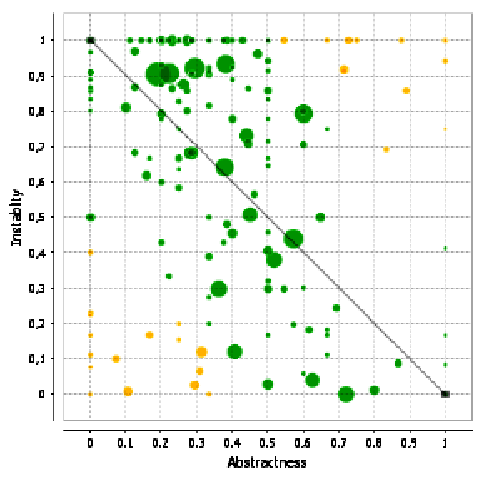
\includegraphics[width=7cm]{figures/martins_metrics2.pdf}
\caption{Příklad grafu závislosti nestability $I$ na abstrakci $A$ \cite{STAN_paper}. Zelené bubliny značí třídy, které jsou blíže diagonále,
zatímco oranžové jsou od ní daleko a nacházejí se v~krajních oblastech, což značí nedodržení SAP. Velikost bublin znázorňuje výsledky metriky SLOC.}
\label{fig:martins_metrics}
\end{center}
\end{figure}

\paragraph{Distance from Main Sequence (D)} je vzdálenost od hlavní diagonály v~grafu závislosti $I$ na $A$.
$$D = A + I - 1$$
$D$ nabývá hodnot z~intervalu $<-1,1>$. Pokud $D = 0$, pak modul leží přímo na diagonále. Čím víc se od ní hodnota $D$ vzdaluje,
tím hůř je architektura systému navržena. Hodnota D může evidentně nabývat dvou mezních hodnot (-1 a 1), což jsou levý dolní
a pravý horní roh grafu. Okolí levého dolního rohu se nazývá \textit{Zone Of Pain} \cite{STAN_paper} a moduly by se v~ní neměly vyskytovat,
protože takový modul je často používaný jinými moduly a není vůbec nebo je pouze minimálně abstraktní, což podle SAP nevěští dobrý návrh.
Stejně tak moduly, které jsou hodně abstraktní a zároveň nejsou jinými moduly používané by se v~systému neměly moc vyskytovat,
protože se nachází v~oblasti pravého horního rohu, které se trefně přezdívá \textit{Zone Of Uselessness} \cite{STAN_paper}.

\section{Existující řešení}
\label{sec:ExistujiciSW}
Systémy pro výpočet softwarových metrik nejsou ve světě softwarového inženýrství žádnou novinkou, protože jich už velké množství existuje.
Většina z~nich ovšem trpí některými nedostatky, které je dělají méně užitečnými. Většinou se jedná o~podporu
jen jednoho nebo dvou vstupních jazyků nebo malého počtu softwarových metrik, které systém počítá.
Některé nástroje ani není možné rozumně rozšiřovat formou modulů. Existují ale i velice dobré programy,
které nabízí širokou škálu jak vstupních jazyků, tak metrik, ale ty jsou většinou komerční a nákup licence
se vyplatí zejména firmám.

\paragraph{C and C++ Code Counter (CCCC)}\cite{cccc} je open-source nástroj pro výpočet metrik (CCN, SLOC, CK a HK) ve zdrojových kódech jazyků C, C++.
Výstup ze systému je v~podobě skupiny několika XML a HTML souborů, které obsahují výsledky analýzy (HTML soubory obsahují data z~XML souborů
zformátovaná přehledně do tabulek).

\paragraph{CppDepend, NDepend a XDepend}\cite{CppDepend,NDepend,XDepend} je skupina komerčních produktů od stejného autora, která nabízí profesionální parametry.
Jedná se o~celá IDE, která podporují výpočet až 82 různých softwarových metrik, dále umožňují práci s~analyzovaným projektem
pomocí CQL\footnote{CQL (Code Query Language \cite{CQL}) je dotazovací jazyk, který umožňuje výběr dat získaný
z~analyzovaného zdrojového kódu podle určitých kritérií. Jedná se o~obdobu jazyka SQL.}, takže je možné filtrovat různé
části kódu kombinováním výsledků několika metrik zároveň. Tyto nástroje také nabízí interaktivní vizualizace závislostí jak na úrovni celých
projektů (grafy závislostí), tak i mezi jednotlivými třídami (matice závislostí). Navíc disponují možností integrace do Visual Studia,
takže lze kód snadno analyzovat přímo při vývoji. To v~čem se tři zmíněné nástroje liší je vstupní jazyk. CppDepend umí analyzovat pouze
zdrojové kódy jazyků C a C++, NDepend provádí analýzu .NETových projektů (jazyky C\# a VB.NET) a XDepend zpracovává kódy psané v~Javě.

\paragraph{CheckStyle \cite{CheckStyle} a PMD \cite{PMD}} jsou open-source nástroje, které jsou si velice podobné. Oba se specializují na statickou
analýzu kódů psaných v~Javě. Jejich zaměření se poněkud liší od většiny programů uvedených v~této kapitole, protože nejsou určeny
na informativní vyčíslení softwarových metrik, případně jejich vizualizaci, ale zabývají se přímo označením míst v~kódu, na kterých se
podle nich vyskyuje chyba. Oba programy tedy hledají spíše bug patterny, nicméně oba umí počítat i několik softwarových metrik.
CheckStyle i PMD na vstupu obdrží výčet pravidel, která chceme kontrolovat a vstupní soubory, na nichž bude analýza prováděna.
Tyto soubory nemusí být zdrojovými soubory v~textové podobě. Oba programy využívají toho, že Java kompiluje do mezikódu \cite{JAVABYTECODE}, takže je možné
kontrolu provádět i na \textit{class} souborech, \textit{JAR} souborech nebo na souborech zkomprimovaných do formátu \textit{ZIP},
protože \textit{JAR} je založen na formátu \textit{ZIP} \cite{JARZIP}.
Výstup z~programů je v~podstatě výpis chyb a varování. Jde o~výsledky analýzy podle kritérií zadaných v~konfiguračním souboru, jenž nebyla dodržena.
Kromě čistě textového výstupu lze získat výstupní data i ve formátech XML nebo HTML.
Oba programy jsou sice aplikace pro příkazovou řádku, ale oba umožňují integraci do několika vývojových prostředí, jako jsou NetBeans, Eclipse
JBuilder a další. Navíc CheckStyle disponuje vlastním GUI rozhraním.
CheckStyle i PMD je možné rozšířit o~vlastní kontroly. Nová pravidla pro PMD se dají psát formou XPath dotazů díky tomu, že naparsovaný
zdrojový kód je ve formě abstraktního syntaktického stromu vyexportovaný do XML a na něm se provádí analýza.
CheckStyle se dá rozšířit napsáním modulu v~Javě s~využitím návrhového vzoru Visitor.

\paragraph{FindBugs}\cite{FindBugs} je další open-source nástroj, který je velice podobný dvěma předchozím (CheckStyle a PMD).
Liší se od nich tím, že se orientuje pouze na hledání bug patternů a softwarové metriky nepočítá.
Dalším rozdílem je, že program není moduly rozšiřitelný a jde o~GUI aplikaci. Navíc disponuje možností spuštění přímo z~webu pomocí Java Web Start.

\paragraph{DMS Software Reengineering Toolkit}\cite{DMS} je kolos mezi všemi ostatními nástroji popsanými v~této práci. Jedná se o~sadu
komerčních nástrojů, které kromě statické analýzy provádí i dynamickou analýzu, překlady z~jednoho jazyka do jiného, generování
překladačů, formátování kódů, apod. Společnost Semantic Designs, Inc., která je autorem tohoto produktu je členem OMG (Object Management Group)
a používá tedy specifikace vydané touto skupinou, např. ASTM (\ref{sec:ASTM}). Kromě spousty dalších zmíněných funkcí, DMS počítá
i softwarové metriky (SLOC, CCN, DECDENS, COMM\%, CK metriky, ...) pro více než 20 programovacích jazyků (C, C++, C\#, FORTRAN,
Java, MATLAB, Pascal, PHP, VB, ...). Navíc lze nechat vykreslit i Control Flow Graphs, Call Graphs, grafy architektury a další.
Zdá se, že DMS má takřka nekonečné možnosti a i přes to je rozšiřitelný o~další funkce a frontendy formou modulů.

\paragraph{GEN++}\cite{GENpp} není program pro výpočet softwarových metrik, nýbrž nástroj na jejich tvorbu.
GEN++ používá \textit{Cfront}, což je frontend pro jazyk C++ napsaný Bjarnem Stroustrupem, takže je možné psát aplikace analyzující zdrojové kódy jazyka C++.
Nástroj funguje tak, že napasruje zdrojový kód a uloží ho do abstraktního syntaktického stromu v~určitém formátu, který je kompatibilní s~dotazovacím frameworkem
\textit{GENOA}, který byl původně vyvynut v~AT\&T Bell Laboratories. Jedná se o~dotazovací jazyk pro syntaktické stromy, podobně jako CQL.
Programy pro analýzu kódu se pak píší v~tomto jazyce, který je svou syntaxí dosti zastaralý
\footnote{Jeho specifikace, která je ke stažení na webu projektu GEN++, je z~roku 1994} (např. oproti zmíněnému CQL)
a ani není na první pohled srozumitelný, protože se v~kódu kombinuje kód skriptu s~navigací stromem.
Zde je ukázka dotazu v~jazyku \textit{GENOA}, který pro každou funkci vypíše počet referencí na globální proměnnou:
\begin{verbatim}
ROOTPROC GlobVarRef
PROC GlobVarRef
ROOT CFile;
{
  LOCAL GNODE fname;
  LOCAL GNODE gcnt;
  <globals
    {Declaration
      (?FunctionDef
        (ASSIGN fname (SLOT id $token))
        (ASSIGN gcnt 0)
        [(?IdName
          <scope
            (?Scope_Extern (ASSIGN gcnt (+ 1 gcnt)))
            (?Scope_Static (ASSIGN gcnt (+ 1 gcnt)))
          >
        )]
        (PRINT stdout "Func %s, %s global references" fname gcnt)
      )
    }
  >
}
\end{verbatim}


\paragraph{JavaNCSS}\cite{JavaNCSS} je konzolová aplikace, která je sice open-source, ale umí počítat velmi málo metrik. Za zmínku stají snad jen CCN a vylepšená SLOC.
Výstup analýzy může být uložen do ASCII, HTML nebo XML. Zajímavost této aplikace tkví v~tom, že výsledky mohou být ukládány i ve formátu SVG.

\paragraph{JDepend}\cite{JDepend} je open-source konzolová aplikace pro analýzu zdrojových kódů Javy, která se specializuje hlavně na hledání závislostí
mezi balíčky. Počítá tedy Martinovy metriky a výsledky ukládá buď v~XML, nebo ve vlastním textovém formátu, ke kterému existuje i GUI nadstavba,
která výsledky zobrazí přehledně v~podobě stromu.

\paragraph{JHawk}\cite{JHawk} je komerční aplikace pro statickou analýzu kódů psaných v~Javě. Program je možné spouštět
v~konzoli, v~samostatném grafickém rozhraní nebo jako součást prostředí Eclipse. JHawk umí počítat širokou
škálu metrik (CCN, SLOC, CK metriky, HK metriky, Halsteadovy metriky, ...). Výstup
z~analýzy může být zobrazen v~grafickém rozhraní ve formě tabulek nebo může být exportován ve formátech
HTML, XML a CSV. Při zakoupení plné licence, obdrží zákazník mimo jiné i zdrojové kódy JHawku (implementováno v~Javě),
takže si ho může sám dál rozšiřovat.

\paragraph{JMetric}\cite{JMetric} je open-source nástroj pro výpočet softwarových metrik (CCN, SLOC, LCOM) na zdrojových kódech psaných v~Javě.
Aplikace umožňuje běh v~příkazové řádce i v~grafickém rozhraní. Výstup je textový, ale lze ho exportovat i do XML a HTML nebo
lze nechat ze získaných hodnot vygenerovat grafy.

\paragraph{McCabe IQ}\cite{McCabeIQ} je produktem společnosti McCabe Software, kterou již před více než 30ti lety založil Thomas J. McCabe,
což je autor definice cyklomatické složitosti CCN. \mbox{McCabe} Software se zabývá dynamickou analýzou, statickou analýzou a bezpečnostní
analýzou a \mbox{poskytuje} širokou škálu služeb včetně možnosti dynamické analýzy na jejich serverech nebo i analýzu webových aplikací.
Produkt McCabe IQ zvládá počítat softarové metriky (SLOC, CCN, CK metriky, HK metriky, Halsteadovy a spoustu dalších) pro zdrojové kódy
velkého počtu jazyků (Ada, ASM86, C, C\#, C++.NET, C++, JAVA, JSP, VB, VB.NET, COBOL, FORTRAN, Perl a PL1). Program se vyznačuje především
tím, že všechny výsledky přehledně vyzualizuje do grafů, které jasně ukazují, jak je analyzovaný projekt implementován a nemůže
tedy dojít k~chybné interpretaci číselných hodnot. Ale i hodnoty lze získat, protože jsou v~grafech uvedeny a navíc je možné z~výsledků
vygenerovat XML report.

\begin{figure}[H]
\begin{center}
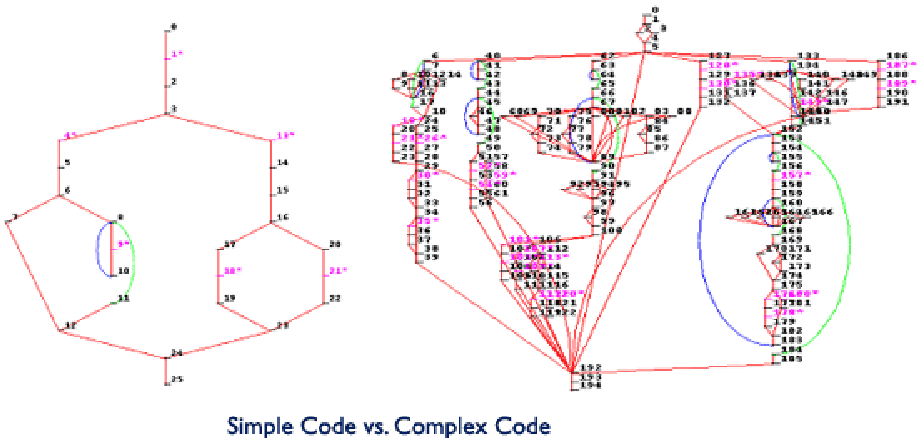
\includegraphics[width=12cm]{figures/mccabe_iq.pdf}
\caption{Ukázka výsledků dvou měření cyklomatické složitosti nástrojem McCabe IQ.}
\label{fig:mccabe_iq}
\end{center}
\end{figure}

\paragraph{Metrics}\cite{Metrics} je open-source plugin do Eclipse, který počítá softwarové metriky (CCN, SLOC, CK metriky, Martinovy metriky, apod.)
pro zdrojové kódy psané v~Javě. Dále umí i vykreslovat grafy závislostí mezi jednotlivými balíčky. Výstup z~analýzy je v~grafické podobě
(využívá rozhraní Eclipse) a je možné nechat si jej vyexportovat do XML.

\paragraph{PHPDepend}\cite{PHPDepend} je odnož projektu JDepend a jde se o~skript pro výpočet softwarových metrik, pomocí kterého lze nechat vyhodnotit kvalitu
zdrojových kódů psaných v~jazyku PHP. PHPDepend umí vypočítat metriky SLOC, CCN, NPath a několik metrik orientovaných na objektový návrh,
včetně Martinových. Výsledky analýzy jsou uloženy do XML souboru. Zároveň s~tím jsou vygenerovány grafy reprezentující výsledky vizuálně.

\paragraph{Project Analyzer}\cite{ProjectAnalyzer} je komplexní komerční nástroj pro vývoj aplikací ve Visual Basicu (VB, VB.NET, VBA). Project Analyzer
obsahuje kromě klasických prvků, jako je editor, kompilátor, apod. i komponentu Project Metrics, díky které lze zjistit výsledky
více než 180ti metrik. Program tyto výsledky dokáže i vykreslovat do přehledných grafů nebo z~nich generovat HTML reporty.

\paragraph{PyMetrics}\cite{PyMetrics} je konzolová aplikace, která analyzuje zdrojové kódy jazyka Python. Umí počítat CCN, SLOC, COMM\% a další.
Výstup analýzy je vypsán do konzole, ale zároveň je vygenerován CSV soubor a skript pro vytvoření SQL tabulek. V~těchto souborech
je uložena rozparsovaná podoba zdrojového kódu, takže je pak možné tuto aplikaci rozšiřovat o~výpočet dalších metrik pomocí
analýzy CSV souboru nebo jednodušeji pomocí SQL dotazů. Nevýhoda tohoto přístupu ale spočívá v~tom, že počítat složitější metriky by bylo
obtížné, protože v~databázi (SQL, CSV) je uložen pouze seznam tokenů, čímž se ztrácí informace o~některých syntaktických a sémantických vazbách, které
by bylo potřeba opakovaně dopočítávat.

\paragraph{Resource Standard Software Source Code Metrics (RSM)}\cite{RSM} je komerční nástroj, který umožňuje výpočet softwarových metrik
(SLOC, CCN, COMM\%, ...) pro jazyky C, C++, C\# a Java. S~programem RSM lze pracovat nejen v~konzoli nebo s~použitím
grafického rozhraní, ale lze ho i integrovat do několika nejpoužívanějších IDE (Visual Studio, JBuilder, Eclipse, ...).
Výsledky analýzy mohou být zobrazeny grafickým rozhraním nebo exportovány do souborů (HTML, XML, CSV).
I~přesto, že je tento software komerční, je možné stáhnout verzi, která je zadarmo a jediným omezením je pouze to, že lze analýzu
provádět na projektech, obsahujích do dvaceti souborů. Prodejce tím chce dát program k~dispozici pro vyzkoušení a pro menší studentské práce.

\paragraph{SourceMonitor}\cite{SourceMonitor} je freeware program s~jednoduchým grafickým rozhraním umožňující výpočet několika základních softwarových metrik
(SLOC, COMM\%, DECDENS, CCN) na zdrojových kódech v~jazycích C, C++, C\#, VB.NET, Java a Delphi. Výsledek analýzy je zobrazen v~tabulce
grafickým rozhraním. Je možné nechat vygenerovat reporty v~XML nebo CSV.

\paragraph{Structural Analysis for Java (STAN)}\cite{STAN} je nástroj pro analýzu zdrojových kódů napsaných v~Javě a pro nekomerční použití je zdarma. Jinak je potřeba
zaplatit licenci. Jedná se o~plugin do vývojového prostředí Eclipse, který je zaměřen především na vizualizaci a hledání závislostí. STAN umí vypočítat i několik
základních metrik jako například počty tříd, funkcí, SLOC, CCN nebo CK metriky.

\paragraph{Testwell tools}\cite{Testwell} je komplexní sada nástrojů pro vyhodnocování kvality software. Jedná se o~komerční produkt, který
je distribuován ve formě programu pro příkazovou řádku, nicméně k~němu existuje i nadstavba v~podobě grafického rozhraní.
Zároveň lze jednotlivé nástroje integrovat do Visual Studia. Testwell tools provádí dynamickou i statickou analýzu a podporují jazyky
C, C++ a Java. Kromě nástroje pro testování a kontrolu code coverage kritéria, je tu i nástroj pro výpočet softwarových metrik
(SLOC, CNN, COMM\%, Halsteadovy metriky a několik dalších). Výstup z~programu může být grafický (při použití nadstavby), textový do konzole
nebo v~podobě reportů (ASCII, HTML, XML, Exel).

\paragraph{Understand}\cite{Understand} je profesionální IDE umožňující podrobnou analýzu zdrojových kódů, které lze v~tomto prostředí rovnou psát, protože
disponuje pokročilým editorem. Understand umí vizualizovat závislosti a počítat přes 70 metrik. Nástroj také podporuje širokou škálu programovacích
jazyků: Ada, C, C++ (bez podpory šablon), FORTRAN, Java, JOVIAL, Pascal, PL/M a VHDL.
Výstup z~analýzy nemusí být pouze vizuální, protože lze nechat generovat i několik typů HTML reportů.

\paragraph{Vil}\cite{Vil} je konzolová utilita, která umožňuje analyzovat .NET a Mono aplikace. Tento program se od ostatních liší tím, že neprovádí
analýzu přímo na zdrojovém kódu, který napsal programátor, ale až na jeho zkompilované verzi. To je možné díky tomu, že .NET i Mono aplikace
nejsou překládány přímo do strojového kódu, ale do tzv. .NET assemblies, což jsou jednotky (exe nebo dll), které obsahují mezikód programu
v~Common Intermediate Language (CIL). Jedná se o~nízkoúrovňový objektově orientovaný programovací jazyk zásobníkového typu, který spadá mezi Assemblery.
Nástroj tak využívá jednoduché gramatiky CIL a toho, že zároveň zachovává informace o~objektech, takže je stále možné počítat některé metriky
a zjišťovat závislosti mezi jednotlivými třídami. Program umí počítat cyklomatickou složitost, CK metriky a Martinovy metriky.
Výsledky analýzy je možno vypsat do konzole nebo je nechat zrofmátovat do XML souboru, či HTML tabulky.

%*****************************************************************************
\chapter{Návrh řešení}
\label{sec:Navrh}

\section{Architektura}
\label{sec:Architektura}
Celý systém se sestává ze tří částí. První z~nich je jádro, které má na starosti propojení a řízení celého systému.
Druhou část tvoří jednotky překladačů (tzv. frontendy), které zpracovávají jednotlivé zdrojové kódy na vstupu systému.
Poslední částí je skupina analytických modulů, které vyhodnocují jednotlivé softwarové metriky pro soubory zdrojových kódů
zpracované vstupními jednotkami.

\begin{figure}[H]
\begin{center}
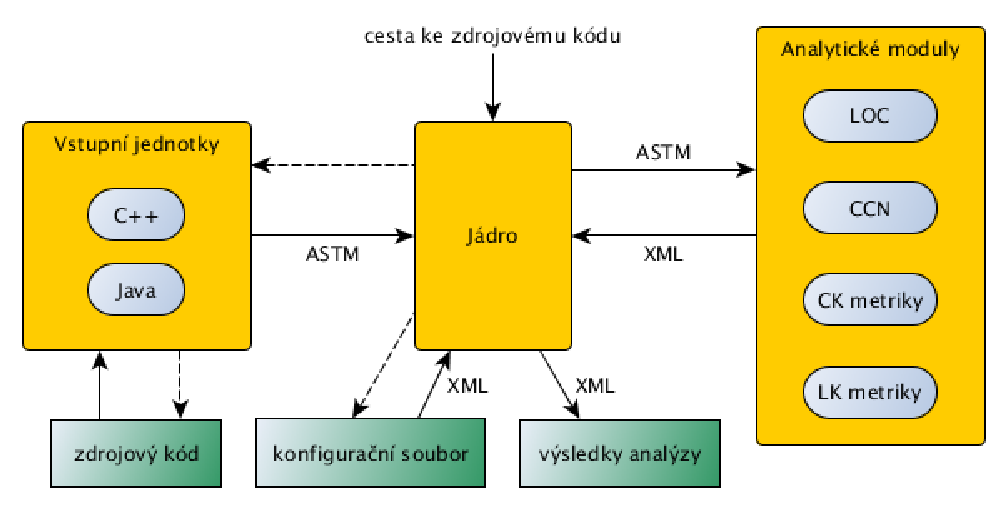
\includegraphics[width=13cm]{figures/architecture.pdf}
\caption{Architektura systému.}
\label{fig:architecture}
\end{center}
\end{figure}

\subsection{Jádro systému}
Jádro je centrálním prvkem celého systému. Jeho hlavním úkolem je zajištění toku dat mezi frontendy a analytickými moduly.
Kvůli tomu je součástí jádra i sada tříd, které reprezentují uzly abstraktního syntaktického uzlu, tzv. ASTM (\ref{sec:ASTM}),
jenž zmíněný tok dat zapouzdřují.

Dalším z~úkolů jádra je zpracování konfiguračních souborů, které řídí jak bude celý systém
kolem jádra poskládán (jaké vstupní jednotky a jaké analytické moduly budou načteny a používány). Konfigurace je v~textovém
formátu, takže uživatel může jeho editací \mbox{kontrolovat} chování systému bez potřeby opětovné kompilace.
Na straně vstupních jednotek je možné v~konfiguraci nastavit asociaci přípon zdrojových souborů ke konkrétnímu frontendu.
U~analytických modulů je možnost nastavit podmíněné použití, což znamená, že lze určit pro jakou
vstupní jednotku bude modul použit a pro jakou se bude tvářit jako neaktivní. To v~praxi znamená, že například pro
jednotku, zpracovávající zdrojové soubory jazyka C, může uživatel vypnout výpočet metrik analyzujících objektový návrh,
jejichž výpočet by stejně kvůli absenci tříd v~C neměly žádný smysl.

\subsection{Vstupní jednotky}
Systém při svém spuštění dostává na vstupu nějaký zdrojový soubor, pro který je potřeba spočítat jednotlivé softwarové metriky.
Aby to bylo možné, je potřeba nejdříve vstupní soubor rozparsovat. O~to se starají právě vstupní jednotky. Typicky jedna jednotka
parsuje jeden jazyk, takže v~systému můžou být například jednotky pro C++, Javu, Fortran a další. Každá taková jednotka se
skládá ze dvou propojených částí, z~nichž první provádí lexikální analýzu a druhá provádí syntaktickou analýzu.
Při lexikální analýze se zdrojový kód převede na sérii lexikálních symbolů, které jsou následně zpracovány podle množiny
pravidel syntaktické analýzy, na jejímž výstupu se nachází tzv. abstraktní syntaktický strom (Abstract Syntax Tree - AST),
který reprezentuje zdrojový kód v~podobě, ve které jsou evidentní veškeré syntaktické a sémantické vazby jednotlivých konstrukcí.
Takový formát je daleko vhodnější pro výpočty jednotlivých softwarových metrik než textová podoba zdrojového kódu.
Vzhledem k~tomu, že AST obecně není nijak blíže specifikovaný, je potřeba zavést jednotný formát pro všechny vstupní jednotky.
Tímto formátem je ASTM (\ref{sec:ASTM}).

\subsection{Analytické moduly}
Všechny analytické moduly musí implementovat rozhraní poskytnuté jádrem systému. Toto rozhraní předepisuje jak moduly komunikují
se zbytkem systému. Modul na vstupu dostává ASTM reprezentující nějaký konkrétní soubor nebo skupinu souborů.
Procházením syntaktického stromu ho modul libovolným způsobem zanalyzuje (provede výpočty pořebné pro vyhodnocení
nějaké metriky, kterou zastupuje) a na výstup vrátí výsledek.

\section{ASTM}
\label{sec:ASTM}
Abstract Syntax Tree Metamodel (ASTM) je formát abstraktního syntaktického stromu \cite{ASTM}, jehož první specifikace byla vydána v~listopadu 2008 sdružením
Object Management Group (OMG) jako jednotný vzor pro tvorby syntaktických stromů v~programech zabývajících se například překladem
z~jednoho jazyka do druhého, vizualizací informací ze zdrojových kódů, refaktorizací, výpočtem softwarových metrik nebo jakoukoli
další analýzou syntaktického stromu. Aktuálně se specifikace tohoto formátu nachází ve verzi je ASTM 1.0 Beta 2, která byla vydána v~červenci 2009.

ASTM je navrženo tak, aby pomocí něj bylo možné uchovávat informace jak syntaktické, tak i sémantické a to z~co největší množiny
vstupních jazyků. Podporovány jsou jazyky druhé (Assemblery), třetí (Fortran, Cobol, Basic, Pascal, C), čtvrté (C++, Java, PHP)
i páté (Prolog, Lisp) generace. V~ASTM lze reprezentovat programy napsané v~jazycích pro strukturované programování stejně tak, jako pro
nestrukturované a funkcionální programování.

%\begin{figure}[H]
%\begin{center}
%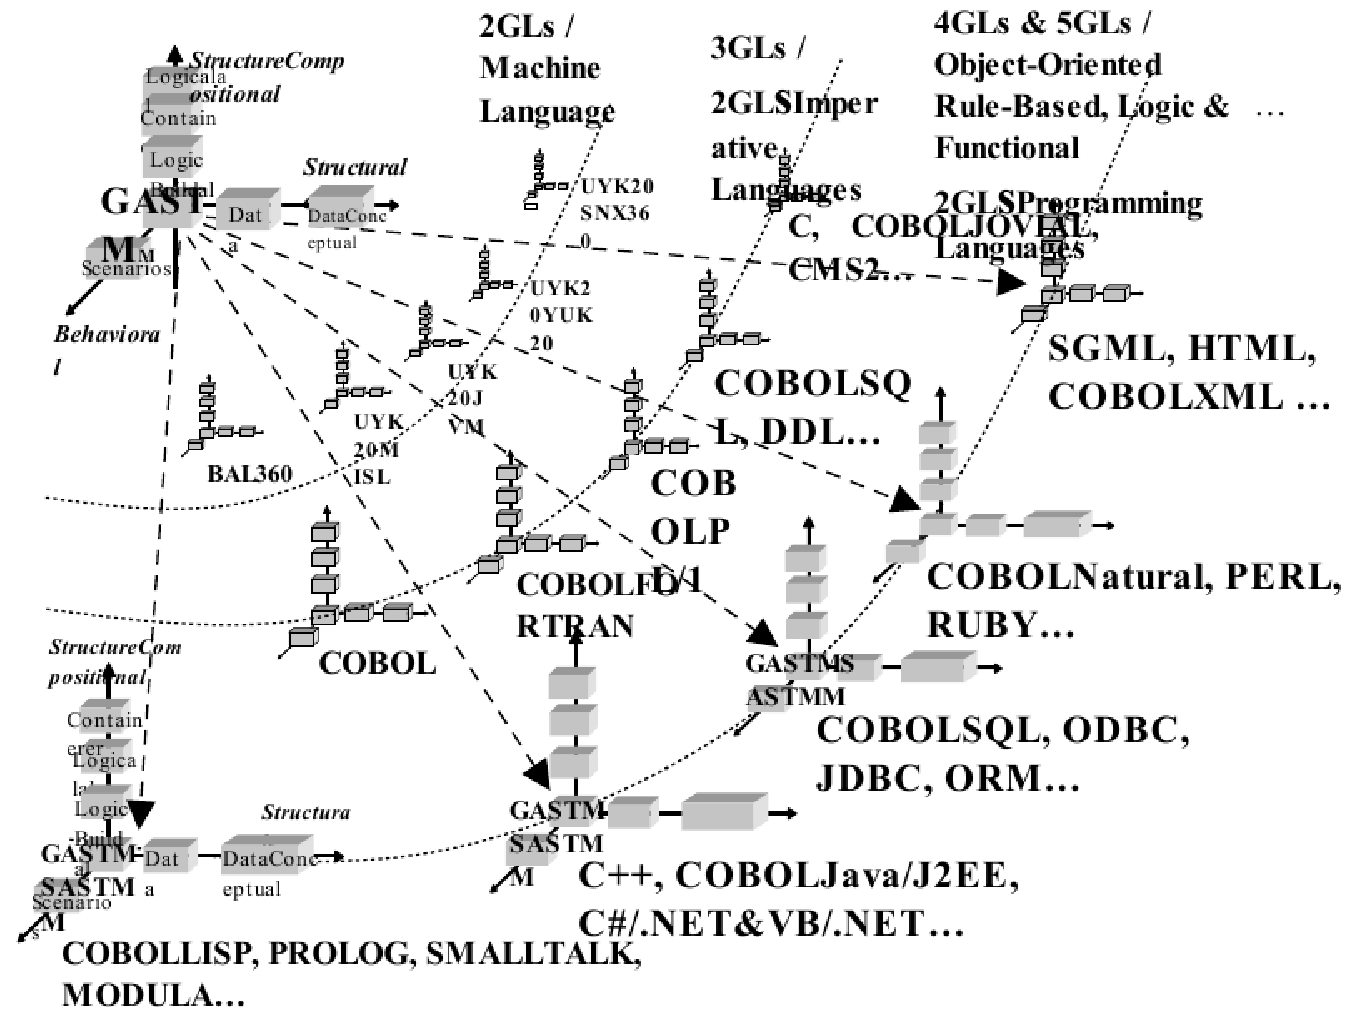
\includegraphics[width=15cm]{figures/lang_generations.pdf}
%\caption{Vývoj programovacích jazyků a jejich podpora v ASTM.}
%\label{fig:lang_generations}
%\end{center}
%\end{figure}

Pro účely tohoto systému byly některé části ASTM navrženy odlišně od specifikace vydané OMG. Důvodem byly některé požadavky na systém,
jako například možnost zjištění, jestli programátor správně odsazuje, což při zachování jednoprůchodové analýzy zdrojového souboru vyžaduje
propojit samotný text zdrojového kódu se stromovou strukturou. Kvůli tomu byly do ASTM přidány například odkazy na tokeny
nebo odkazy na rodičovské uzly, takže tíky tomuto je možné procházet zdrojový kód, který je uložen v~obousměrném spojovém seznamu jako seznam tokenů,
kde každý z~nich navíc obsahuje informaci o~své pozici v~souboru a také odkaz na uzel stromu, který konkrétní token nebo více tokenů reprezentuje.
Tato struktura umožňuje nejen procházení stromu od jeho kořene do listů, ale i obráceně od listů do kořene, což má za následek spoustu možností
pro následnou analýzu.

\begin{figure}[H]
\begin{center}
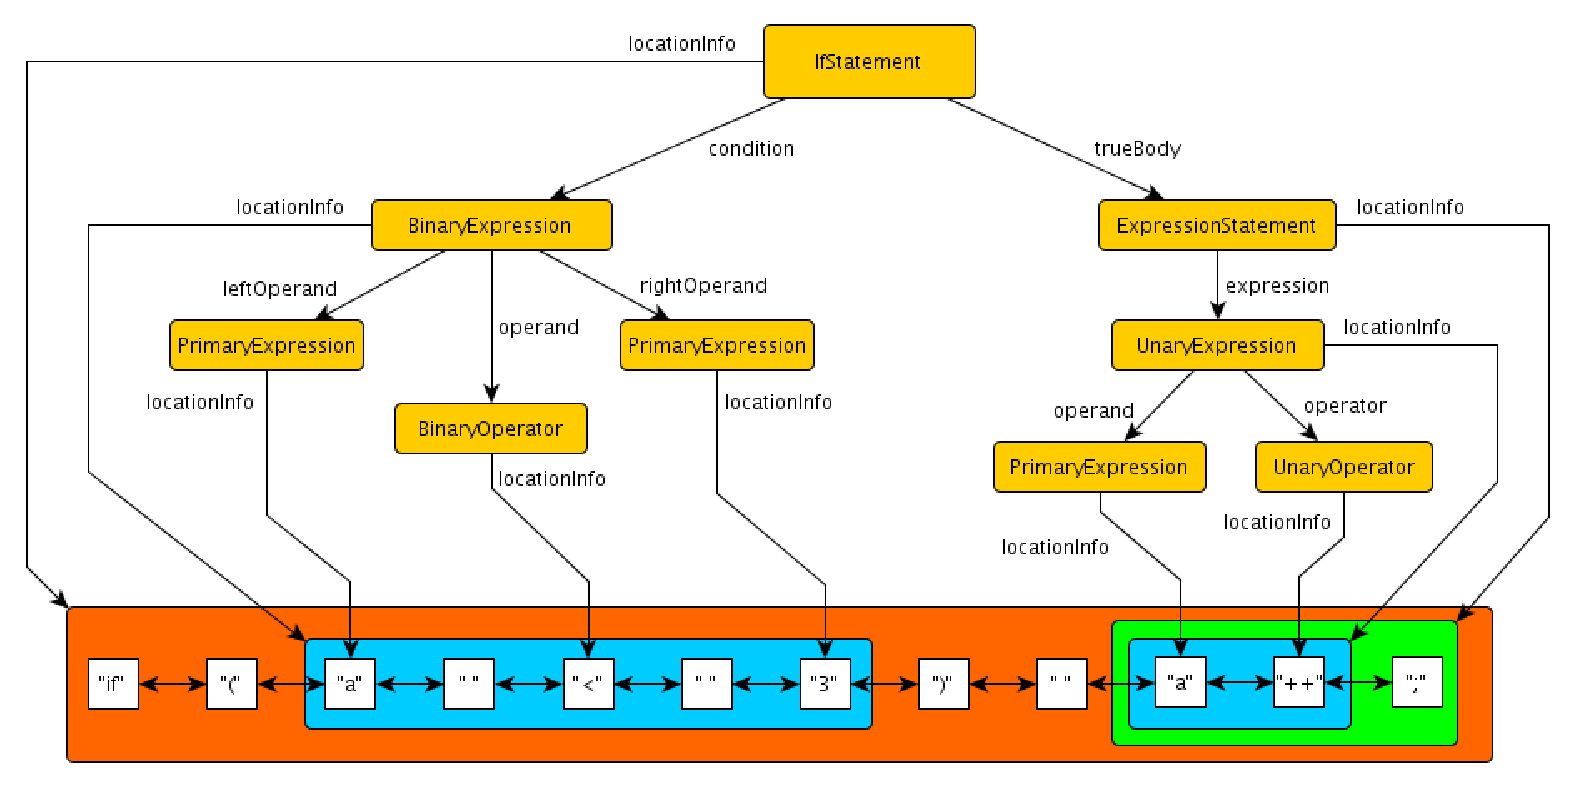
\includegraphics[width=15cm]{figures/parsing_example.pdf}
\caption{Ukázka, výsledku parsování do ASTM pro úryvek kódu: \textit{if(a < 3) a++;}. \mbox{Poznámka:} \textit{obrázek je pouze ilustrační,
aby bylo zřejmé, jak je strom konstruován, takže jsou v~něm některé údaje a vazby vynechány}.}
\label{fig:parsing_example}
\end{center}
\end{figure}

\section{Životní cyklus aplikace}
\begin{enumerate}
 \item Systém dostane na vstupu jméno souboru, který chce uživatel nechat analyzovat.
 \item Jádro podle přípony souboru a podle konfigurace vyhodnotí kterému frontendu soubor náleží.
 \begin{enumerate}
  \item Jestliže soubor nenáleží žádnému aktivnímu frontendu, je program ukončen.
 \end{enumerate}
 \item Jádro zavolá příslušný frontend a vyžádá si od něj ASTM.
 \item Frontend vytvoří ASTM reprezentující zdrojový kód předloženého souboru a předá ho jádru.
 \begin{enumerate}
  \item Pokud zdrojový soubor neexistuje nebo pokud obsahuje chyby (syntaktické, sémantické), je program ukončen.
 \end{enumerate}
 \item Jádro zjistí, které analytické moduly jsou aktivní pro daný typ zdrojového souboru.
 \item Jádro postupně zavolá všechny moduly, které jsou aktivní. Každý modul na vstupu dostane ASTM a očekává se, že vrátí informace o~výsledku analýzy.
 \item Moduly prochází ASTM, provádí analýzu a vrací její výsledek zpět do jádra. V~průběhu analýzy není do ASTM zasahováno.
 \item Po ukončení práce všech analytických modulů jsou výsledky analýzy, které jádro posbíralo od svých modulů, uloženy do reportu a program je ukončen.
\end{enumerate}

%*****************************************************************************
\chapter{Realizace}
\label{sec:Realizace}
Celý systém pro výpočet softwarových metrik je implementován v~jazyku C++ a funguje na všech platformách, kde se
k~dispozici překladač jazyka C++ a nástroje Flex a Bison (viz níže).

Systém je momentálně vybaven pouze jedním frontendem, který zpracovává zdrojové soubory jazyka C++. Frontend implementuje
gramatiku podle normy ANSI/ISO C++ z~roku 2003 \cite{ISOCpp03}. V~současném stádiu vývoje je podporována pouze podmnožina možností, kterými
jazyk C++ podle této normy disponuje. V~implementaci chybí zejména podpora direktiv preprocesoru, šablon a rozlišování oborů platnosti
proměnných pomocí operátoru \textit{::}. Dále není implementováno přetěžování operátorů a operátory \textit{new} a \textit{delete}.
Na to se vážou důsledky takovéto neúplné implementace, jako je například nemožnost includovat hlavičkové soubory a tedy není možné
správně sémanticky identifikovat některé funkce, objekty, typy, případně jmenné prostory deklarované mimo analyzovaný soubor.
Frontend podporuje zejména základní kontrukce jazyka C++, aby bylo možné počítat některé softwarové metriky představené v~kapitole \ref{sec:KvalitaKodu}.
Podporovány jsou tedy běžné stavební kameny většiny programovacích jazyků, jako jsou podmínky, cykly, funkce, primitivní datové typy,
jmenné prostory a třídy včetně dědicnosti.

Frontend je realizován GNU nástroji \textbf{Flex} \cite{Flex} a \textbf{Bison} \cite{Bison}.

\paragraph{Flex} byl použit pro vygenerování lexikálního analyzátoru. Zdrojový skript pro Flex obsahuje regulární výrazy, pomocí nichž
jsou jednotlivé podřetězce analyzovaného zdrojového kódu vyhodnocovány jako tokeny. Tokeny z~lexikální analýzy mají podobu objektu, který
obsahuje identifikaci toho o~jaký typ tokenu se jedná, řetezec, který jej tvoří a také informaci o~přesné pozici tokenu ve zdrojovém kódu.
Výsledný objekt je předán dále ke zpracování parseru\footnote{Parser = syntaktický analyzátor.}.

\paragraph{Bison} generuje syntaktický analyzátor ze skriptu, který obsahuje gramatická pravidla jazyka C++ podle již zmíněné normy ANSI/ISO C++ z~roku 2003.
Tento skript navíc obsahuje i funkce pro sémantickou analýzu, protože gramatika tohoto jazyka obsahuje spoustu kolizí, které je potřeba při analýze vyřešit.
Drtivá většina těchto kolizí je zapříčiněná tím, že je gramatika pojata \uv{sémanticky}, tzn. že například identifikátor je v~jednom pravidle pojmenován jako
jméno třídy (\textit{class-name}), v~jiném pravidle zase jako jméno funkce (\textit{unqualified-id}), apod. Stejná je situace se šablonami, jmenými prostory, atd.
Ve výsledku jde vždy o~stejný typ tokenu a parser se nedokáže rozhodnout mezi dvěma takovými pravidly. Zde přichází na řadu sémantika.

Bison typicky generuje tzv. LALR parser (Look-Ahead Left-to-right Rightmost derivation parser), který pro sémantickou analýzu sice není nevhodný,
ale problém je ve způsobu, jakým Bison zpracovává vstupní gramatiku, protože je prakticky nemožné do ní přidat sémantická pravidla tak,
aby se na kolizi aplikovala včas, tzn. ještě před tím než je token zahozen. Zde se dá využít možnost Bisonu, aby generoval GLR parser
(Generalized Left-to-right Rightmost derivation parser). Tento typ parseru má tu výhodu, že pokud se v~gramatice vyskytne kolize,
probíhá analýza paralelně pro každou variantu a když se některá z~nich díky následujícím tokenům prokáže jako špatná, je vyřazena ze zpracování.
Potom můžou nastat dvě situace. První z~nich je ta, že zbyde pouze jedna varianta a ta je správná. Druhá situace nastane, když zůstane
víc větví a ty se opět spojí do jedné (tzv. merge). V~tom případě je potřeba využít sémantiku, takže se prohledá tabulka symbolů a určí se,
zda se jedná o~funkci, třídu, či něco jiného. Špatné větve se pak zahodí a pokračuje se pouze v~těch, které zbyly. Na konci analýzy zbyde vždy jen
jedna větev, která je správná (pokud nedošlo k~syntaktické nebo sémantické chybě).

Výsledný parser na vstupu dostává objekty reprezentující tokeny přečtené ze zdrojového kódu lexikálním analyzátorem a podle
syntaktických a sémantických pravidel vytváří abstraktní syntaktický strom (ASTM), který reprezentuje analyzovaný zdrojový kód.

Kromě frontendu pro C++ obsahuje systém i jádro a moduly pro výpočet jednotlivých softwarových metrik, jak bylo popsáno v~návrhu architekruty (\ref{sec:Architektura}).
Jádro je prostředníkem mezi frontendy a analytickými moduly.

\paragraph{Výstup systému} je realizován ve formě XML souboru, který obsahuje výsledky softwarových metrik pro analyzovaný zdrojový soubor.
V~systému jsou momentálně implementovány moduly pro metriky SLOC, COMMDENS, CCN, DECDENS, NPATH, TFC, NOC a LK. Bližší informace
o~jejich výpočtu jsou v~kapitole \ref{sec:Testovani}. Na výsledný XML soubor může být následně aplikována přiložená XSL šablona,
která výsledky formátuje přehledně do tabulek.

%K výslednému programu je přiložena dokumentace vygenerovaná nástrojem Doxygen s použitím knihovny Graphviz pro vizualizaci hirarchie třid.
%Celý systém je sestaven systémem CMake.

%*****************************************************************************
\chapter{Testování}
\label{sec:Testovani}

\section{C++ frontend}
Jak už bylo zmíněno v~kapitole \ref{sec:Realizace}, k~implementaci frontendu byly použity nástroje Flex a Bison, což
značně omezuje nutnost kontroly chyb, oproti ručně psaným překladačům. Důležitým prvkem je však testování
sémantiky, na které je závislá veškerá další analýza. Zdrojový kód je parsován a ukládán
do abstraktního syntaktického stromu (ASTM, viz kapitola \ref{sec:ASTM}), jehož všechny uzly jsou obohaceny o~funkce generující výstup ve formátu
XML. Když je pak na kořen stromu zavolána zmíněná funkce, rekurzivně se vytvoří XML dump celého stromu.
Dump obsahuje {veškerá data}\footnote{Vynechány jsou pouze křížné reference mezi některými uzly, což by jinak vedlo k~zacyklení.}, jenž jsou v~uzlech uložena.
Díky tomu se dá frontend testovat dvěma způsoby. Prvním je procházení stromu přímo v~paměti a druhým je kontrola vytvořeného XML souboru, jenž daný strom reprezentuje.
Výhoda takového řešení je velká, protože v~XML souboru je na první pohled jasně vidět, jak je strom vytvořen, zatímco v~paměti je toto hodně složité
a to i s~výbornými debuggery, jako má například VisualStudio. Zároveň se do velké míry jedná i o~dokumentaci frontendu, protože stačí
pohled do vygenerovaného XML souboru a hned je jasné, jak strom vypadá a není potřeba zdlouhavě studovat dokumentaci ASTM\footnote{Navíc ani ta negarantuje, že byl podle ní strom vytvořen.}.
Lze také použít nástroje pro práci s~XML, kterými je možné strom vizualizovat (díky standardu XML DOM).

Samotná kontrola struktury stromu byla realizována právě pomocí XML souboru. Na něj byly aplikovány XSL šablony, které provádí kontroly
a zároveň přehledně vykreslují výsledky.

K~programu je přiložena sada XSL šablon, které mají psaní dalších testů usnadnit.
Díky nim stačí vytvořit prázdnou šablonu, zadat XPath výrazy kontrolující nějaké části stromu a vložit předpřipravenou šablonu, z~níž se pak volají
funkce starající se o~vyhodnocení testů.

\begin{figure}[H]
\begin{center}
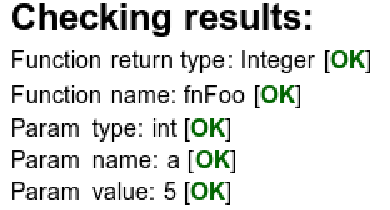
\includegraphics[width=5cm]{figures/testing.pdf}
\caption{Ukázka testování deklarace funkce pomocí XSL šablony aplikované na XML dump syntaktického stromu.}
\label{fig:testing}
\end{center}
\end{figure}

\section{Výpočet softwarových metrik}

\subsection{SLOC}
Výsledkem této skupiny metrik je informace o~počtu všech řádků (LOC),
počtu rádků na nichž se vyskytuje komentář (CLOC) a o~počtu řádků, na kterých je
nějaký výkonný kód (LLOC), tzn. řádek není prázdný nebo na něm není pouze komentář.
Například následující řádek
\begin{verbatim}
int a;	// deklarace a
\end{verbatim}
je započítán jako LOC, LLOC i CLOC.
Výsledky metrik udávají počty řádků pro celý soubor a pak zvlášť pro každou definici funkce.
Správnost výsledků byla ověřována manuálně i porovnáním s~výstupem z~programu CCCC, se kterým se výsledky shodovaly.

\begin{figure}[H]
\begin{center}
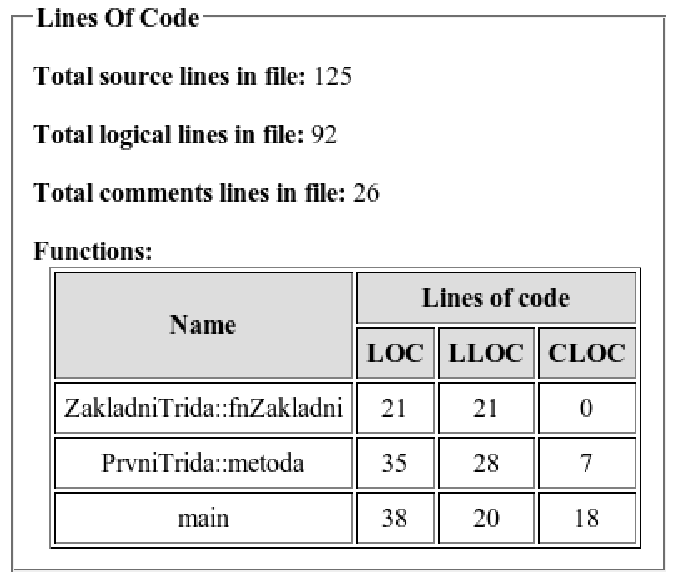
\includegraphics[width=9cm]{figures/output_sloc.pdf}
\caption{Ukázka výstupu z~modulu pro výpočet SLOC metrik.}
\label{fig:out_sloc}
\end{center}
\end{figure}

\subsection{COMMDENS}
Tato metrika byla uvedena v~kapitole Comments Density (\ref{sec:MCOMM}) a určuje hustotu komentářů.
Způsob výpočtu se neshoduje s~definicemi v~kapitole \ref{sec:MCOMM}, protože první způsob (COMM\%)
je nepřesný kvůli započítávání prázdných řádků a druhý způsob (MCOMM\%) je poměrně složitý v~tom ohledu,
že je dosti sporné, co lze určit za smysluplný komentář. Dalším důvodem je, že z~výsledků SLOC metrik
je snadné použít hodnotu CLOC, takže COMMDENS se dá vypočítat jako poměr počtu řádků obsahující komentáře
ku počtu všech řádků.
$$COMMDENS = CLOC / LOC$$
Výsledkem je pak procentuální vyjádření hustoty komentářů zvlášť pro každou definici funkce.

\begin{figure}[H]
\begin{center}
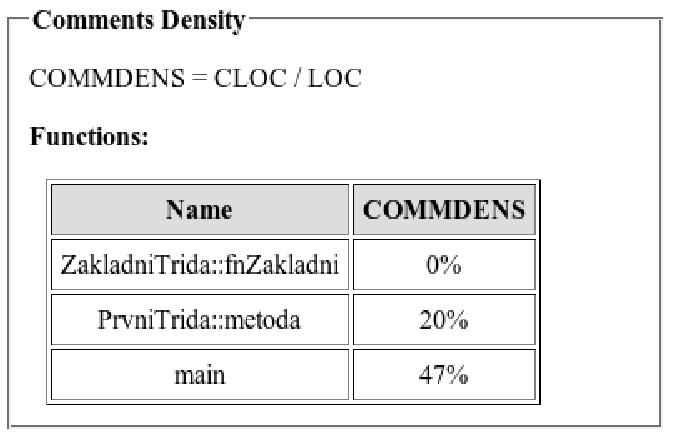
\includegraphics[width=9cm]{figures/output_commdens.pdf}
\caption{Ukázka výstupu z~modulu pro výpočet COMMDENS metriky.}
\label{fig:out_commdens}
\end{center}
\end{figure}

\subsection{CCN}
\label{sec:TestovaniCCN}
Modul pro výpočet CCN se řídí definicí McCabovy složitosti (\ref{sec:CCN}). Kromě výpočtu CCN1, který odpovídá původní definici,
je implementováno i CCN2, které navíc počítá složitost složených výrazů. Výsledky výpočtu byly porovnávány s~nástrojem CCCC.
Ten počítá pouze CCN2 a označuje ji zkratkou MVG (McCabe's $V(G)$). Velkým rozdílem ve výpočtu CCN2 a MVG je odlišná interpretace toho, co je cyklomatická složitost.
CCCC do ní počítá i \textit{break}, \textit{continue}, \textit{goto}, \textit{return} a vyjímky.
Stejně se chovají i jiné nástroje. Například skupina CppDepend, NDepend a XDepend, které se od CCCC liší akorát tím, že nezapočítávají \textit{break}.

Důvodem, proč CCN modul tyto konstrukce nezapočítává je fakt, že kvůli nim se program nevětví, ačkoli je zřejmé, že složitost programu
se jimy zvyšuje. Ovšem při započítání těchto prvků se přestává jednat o~cyklomatickou složitost.
Program se větví, jestliže se v~některém jeho místě rozhoduje, zda půjde jednou cestou, nebo druhou cestou.
Tomu se tak ale při konstrukcích typu \textit{return}, \textit{break}, \textit{continue} a \textit{goto} neděje, protože se jedná o~nepodmíněné skoky.
Stejná je situace s~vyjímkami, protože větvení nastává přímo u~rozhodnutí, zda bude vyjímka vyhozena, či nikoli. Ne při jejím zpracování.

\begin{figure}[H]
\begin{center}
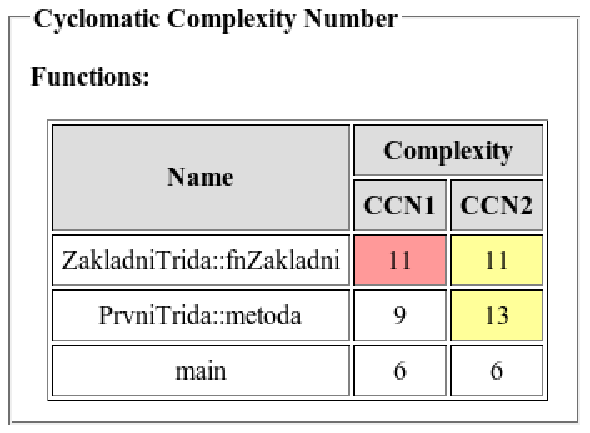
\includegraphics[width=8cm]{figures/output_ccn.pdf}
\caption{Ukázka výstupu z~modulu pro výpočet CCN metrik.}
\label{fig:out_ccn}
\end{center}
\end{figure}

\subsection{DECDENS}
DECDENS, neboli Decision Density je vypočítána přesně podle definice v~kapitole \ref{sec:DECDENS}, tedy
$$DECDENS = CCN / LLOC.$$
Vzhledem k~tomu, že DECDENS má odpovídat hustotě větvících konstrukcí hlavně z~vizuálního hlediska (když se na kód podíváme),
tak se za $CCN$ považuje hodnota $CCN1$ z~předchozí kapitoly \ref{sec:TestovaniCCN}.
Výsledky jsou uváděny zvlášt pro každou definici funkce.

\begin{figure}[H]
\begin{center}
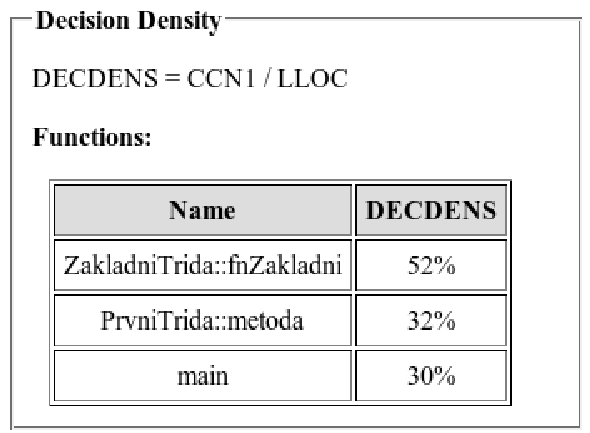
\includegraphics[width=8cm]{figures/output_decdens.pdf}
\caption{Ukázka výstupu z~modulu pro výpočet DECDENS metriky.}
\label{fig:out_decdens}
\end{center}
\end{figure}

\subsection{NPATH}
Výstup z~modulu pro výpočet NPATH, udává složitost funkce přesně podle toho, jak byla definována v~kapitole \ref{sec:NPATH}.
Stejně jako u~výpočtu CCN (\ref{sec:TestovaniCCN}) je zachován způsob výpočtu z~původní definice a nejsou do ní započítávány vyjímky a nepodmíněné skoky.

\begin{figure}[H]
\begin{center}
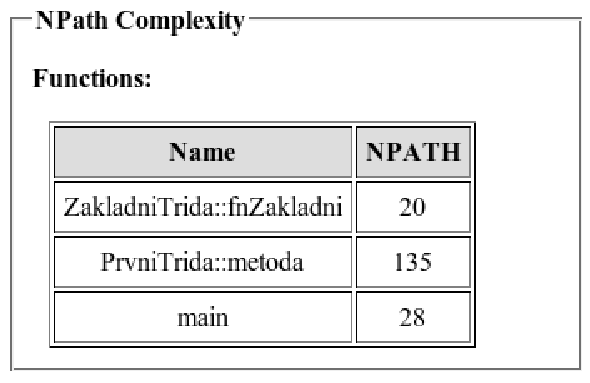
\includegraphics[width=7cm]{figures/output_npath.pdf}
\caption{Ukázka výstupu z~modulu pro výpočet NPATH metriky.}
\label{fig:out_npath}
\end{center}
\end{figure}

\subsection{TFC}
TFC, neboli Total Funcion Calls, udává počet všech volání funkcí, uvnitř zkoumané funkce.
Jedná se o~obdobu \textit{fan-in} z~HK metriky (\ref{sec:HK}).

\begin{figure}[H]
\begin{center}
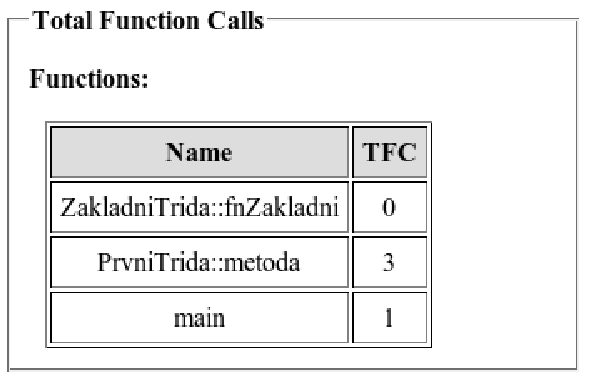
\includegraphics[width=7cm]{figures/output_tfc.pdf}
\caption{Ukázka výstupu z~modulu pro výpočet TFC metriky.}
\label{fig:out_tfc}
\end{center}
\end{figure}

\subsection{NOC}
NOC je zkratkou pro Number Of Classes a udavá celkový počet tříd v~analyzovaném souboru.

\begin{figure}[H]
\begin{center}
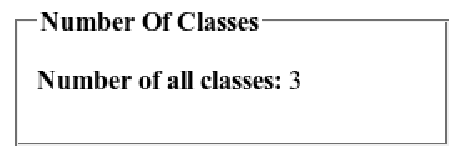
\includegraphics[width=6cm]{figures/output_noc.pdf}
\caption{Ukázka výstupu z~modulu pro výpočet NOC metriky.}
\label{fig:out_noc}
\end{center}
\end{figure}

\subsection{LK}
Modul pro výpočet Lorenz-Kidd (LK) metrik se snaží držet definice z~kapitoly (\ref{sec:LK}).
Bohužel z~definice není úplně jasné, zda se například do počtu všech metod (NM) započítávají
i ty zděděné, nebo ne. Vzhledem k~tomu, že LK metriky se vyloženě zabývají dědičností,
byla zvolena varianta, že se zděděné metody započítávají. Takže například při výpočtu
NM se nejdříve projde strom dědičnosti a podle toho, jakým způsobem jsou jednotlivé třídy děděny
(\textit{private}, \textit{protected}, \textit{public}) a podle toho, jak jsou deklarovány
(opět \textit{private}, \textit{protected}, \textit{public}), je sestaven seznam všech metod,
které se do NM započítají. Modul zároveň dokáže zjistit, zda nějaká funkce zastiňuje zděděnou
funkci předka. Pak je funkce do NM započítána pouze jednou. Výpočet dalších hodnot LK metriky
je pak analogický k~tomuto.

Modul se řídí pravidly pro dědičnost jazyka C++. To znamená, že
metody a atributy se dědí tehdy, když jsou deklarovány jako \textit{protected}
nebo \textit{public} a zároveň dědičnost není typu \textit{private}.
Modul se zatím nedovede vypořádat s~takovým dědědím, kde se v~potomkovi děděné metodě nebo atributu změní typ přístupu na \textit{private}.
To podle normy znamená, že tato metoda už dále děděna není. Nicméně v~modulu se stále považuje za děditelnou.

Vzhledem k~tomu, že se nepodařilo získat nástroj, který by LK metriky počítal, nebylo možné porovnání výsledků.
Většina nástrojů, jejichž dokumentace uvádí, že tyto metriky počítají, lžou, protože počítají například jen počet metod a počet atributů.
Ostatní metriky ignorují. S~tím asi souvisí i fakt, že do počtu metod a atributů
započítávají pouze prvky z~konkrétní třídy a dědičnost se nebere v~úvahu. To je pochopitelné, protože
když nejsou tyto metriky označeny souhrně jako součást LK metrik, pak by výsledky byly matoucí
a zdánlivě by nedávaly smysl.

\begin{figure}[H]
\begin{center}
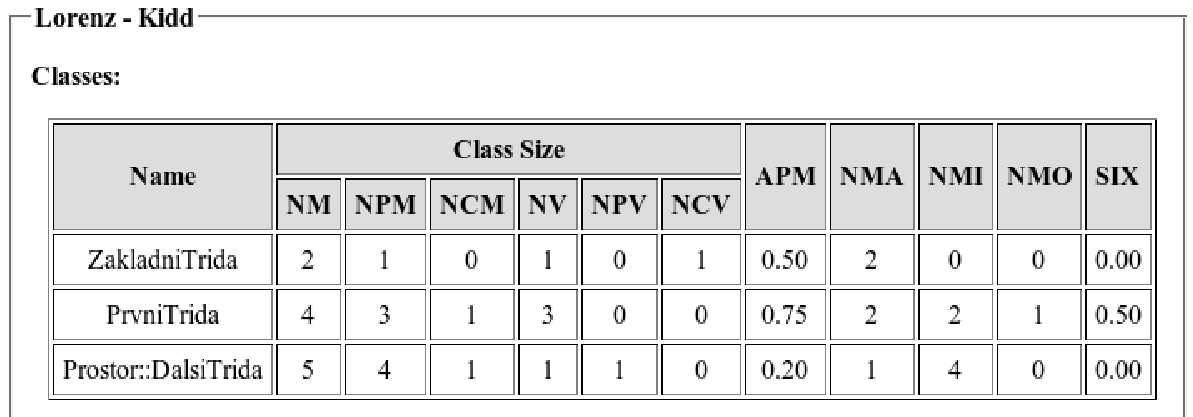
\includegraphics[width=15cm]{figures/output_lk.pdf}
\caption{Ukázka výstupu z~modulu pro výpočet LK metrik.}
\label{fig:out_lk}
\end{center}
\end{figure}



%*****************************************************************************
\chapter{Závěr}

Softwarové metriky představené v~textu jsou užitečné, pokud chceme získat objektivní náhled na kvalitu implementace určitého problému.
Jejich výsledky je ale třeba brát s~rezervou, protože jsou pouze orientační. I~když se díky nim dají najít trhliny v~návrhu,
implementaci nebo testování, bylo by chybou nechat se jimi řídit natolik, že by implementace s~nelichotivým výsledkem nějaké metriky
byla zamítnuta jako nepřípustná, aniž by se člověk podíval do kódu. Stejně tak není možné prohlásit, že je nějaká metrika nejlepší,
řídit se pouze jejími výsledky a ostatní ignorovat. Proto většina nástrojů pro hodnocení kvality kódu poskytuje výpočet více
druhů metrik, aby bylo možné na kód nahlížet z~různých úhlů.

Metriky uvedené v~textu samozřejmě nejsou jediné, které existují. Je jich nepřeberné množství, protože způsobů,
jak nahlížet na kvalitu kódu je spousta. Také u~většiny metrik existuje spousta jejich variant, které se liší. Příkladem budiž
metriky CCN a LCOM, které po svém uvedení doznaly poměrně velkého počtu modifikací několika jinými autory. LCOM
dokonce stojí za vznikem celé skupiny tzv. kohezních metrik.

Výsledkem implementační části práce je systém pro výpočet softwarových metrik, který podporuje výpočet několika metrik
(SLOC, COMMDENS, CCN, DECDENS, NPATH, TFC, NOC a LK) na zdrojových kódech jazyka C++, což bylo zadáním práce. Nicméně pro použití v~reálných
podmínkach není program připraven, protože některé části gramatiky jazyka C++ zatím nebyly implementovány (viz kapitola \ref{sec:Realizace}).
Program také umí analyzovat zdrojové soubory pouze po jednom, což je pro větší projekty nepraktické z~toho důvodu, že by výsledky
analýzy nebyly přístupné pro celý projekt na jednom místě a nebyly by patřičně provázané.

Výsledný systém je možný velice snadno rozšířit o~vstupní jednotky i analytické moduly. Jedná se o~výhodu oproti jiným již existujícím řešením,
které buď rozšířít nejdou nebo je potřeba nastudovat jejich verzi abstraktního syntaktického stromu a navíc rozhraní, které k~psaní rozšíření
poskytují. Pro rozšíření tohoto systému je sice také nutná znalost struktury syntaktického stromu (formát ASTM, viz kapitola \ref{sec:ASTM}),
jehož dokumentace je k~programu přibalena, ale pozitivem je, že jde o~nastupující otevřený standard, který vydala Object Management Group.
Ta také poskytuje podrobnou specifikaci formátu. Další výhodou oproti většině existujících řešení je to, že lze ve stromu pracovat
i se samotným zdrojovým kódem a není k~tomu potřeba žádný průchod souborem navíc. Díky tomu je možné provádět například i analýzu toho,
jak se v~kódu odsazuje, což většina existujících řešení neumí. I~když je program zaměřen na výpočet softwarových metrik,
lze k~němu napsat moduly na hledání bug patterns, kontroly konvencí v~pojmenování, odsazování, apod. Stejně tak není vyloučena možnost dynamické analýzy.

Další vývoj programu bude zaměřen na dokončení frontendu pro jazyk C++ a přidání podpory pro některé další jazyky, například pro Javu.
Postupně budou přibývat i moduly pro výpočet dalších softwarových metrik. Vzhledem k~tomu, že cílem projektu je, aby byl výsledný systém
co nejsnadněji rozšiřitelný, bylo by vhodné, aby se moduly načítaly dynamicky za běhu z~externích knihoven, protože nyní se při přidání
modulu musí celý systém překompilovat. Další možností, jak systém dál rozřířit je například podpora souborů Makefile nebo projektů VisualStudia
a dalších IDE, což by uživateli umožnilo snadnější práci s~programem při analyzování celých projektů.
%Kdyby bylo potřeba, je také možné paralelizovat jednotlivé úkony systému, takže by bylo možné vytvořit přímo server pro vyhodnocování kvality kódu.

%*****************************************************************************
% Seznam literatury je v samostatnem souboru reference.bib. Ten
% upravte dle vlastnich potreb, potom zpracujte (a do textu
% zapracujte) pomoci prikazu bibtex a nasledne pdflatex (nebo
% latex). Druhy z nich alespon 2x, aby se poresily odkazy.

\bibliographystyle{abbrv}
%bibliographystyle{plain}
%\bibliographystyle{psc}
{
%JZ: 11.12.2008 Kdo chce mit v techto ukazkovych odkazech take odkaz na CSTeX:
\def\CS{$\cal C\kern-0.1667em\lower.5ex\hbox{$\cal S$}\kern-0.075em $}
\bibliography{reference}
}


%*****************************************************************************
\chapter{Seznam použitých zkratek}

\begin{description}
\item[.NET] Microsoft .NET Framework
\item[A] Abstractness
\item[AHF] Attribute Hiding Factor
\item[AIF] Attribute Inharitance Factor
\item[ANSI] American National Standards Institute
\item[APM] Average Parameters per Method
\item[AST] Abstract Syntax Tree
\item[ASTM] Abstract Syntax Tree Metamodel
\item[Ca] Afferent Coupling
\item[CBO] Coupling Between Object classes
\item[CCCC] C and C++ Code Counter
\item[CCN] Cyclomatic Complexity Number
\item[CD] Compact Disc
\item[Ce] Efferent Coupling
\item[CFG] Control Flow Graph
\item[CIL] Common Intermediate Language
\item[CK] Chidamber-Kemerer
\item[CLF] CLustering Factor
\item[COCOMO] the COnstructive COst MOdel
\item[COF] Coupling Factor
\item[COMM] COMMent
\item[CS] Class Size
\item[CSV] Comma Separated Values
\item[D] Distance from main sequence (Martin's Package Metrics), případně Difficulty (Halstead's Metrics)
\item[DECDENS] DECision DENSity
\item[DIT] Depth Inharitance Tree
\item[DLL] Dynamic Loaded Library
\item[DOM] Document Object Model
\item[E] Effort
\item[EXE] EXEcutable
\item[Flex] Fast LEXical analyzer
\item[GNU] GNU's Not Unix
\item[HK] Henry-Kafura
\item[HTML] HyperText Markup Language
\item[I] Instability
\item[IQ] Intelligence Quotient
\item[ISO] International Organization for Standardization
\item[JAR] Java ARchive
\item[LCOM] Lack Cohencion Of Methods
\item[LK] Lorenz-Kidd
\item[LLOC] Logical Lines Of Code
\item[LOC] Lines Of Code
\item[MCOMM] Meaningful COMMents
\item[MHP] Method Hiding Factor
\item[MIF] Method Inharitance Factor
\item[MOOD] Metrics for Object Oriented Design
\item[MOOSE] Metrics for Object-Oriented Software Engineering
\item[MVG] McCabe's $V(G)$
\item[NASA] National Aeronautics and Space Administration
\item[NCM] Number of Class Methods
\item[NCV] Number of Class Variables
\item[NM] Number of Methods
\item[NMA] Number of Methods Added
\item[NMI] Number of Methods Inherited
\item[NMO] Number of Methods Overridden
\item[NOC] Number Of Children
\item[NPM] Number of Public Methods
\item[NPV] Number of Public Variables
\item[NV] Number of Variables
\item[OMG] ObjectManagement Group
\item[RF] Reuse Factor
\item[RFC] Response For a Class
\item[PHP] Hypertext Preprocessor
\item[POF] POlymorphism Factor
\item[RSM] Resource standard software Source code Metrics
\item[SAP] Stable Abstractions Principle
\item[SIX] Specialization IndeX
\item[SLOC] Source Lines Of Code
\item[STAN] STructural ANalysis for Java
\item[SVG] Scalable Vector Graphics
\item[TFC] Total Function Calls
\item[WMC] Weight Methods per Class
\item[XML] eXtensible Markup Language
\item[XSL] eXtensible Stylesheet Language
\end{description}

%*****************************************************************************
\chapter{Instalační a uživatelská příručka}

\section{Návod pro instalaci na OS Linux}

\paragraph{Vyzkoušeno s:}
\begin{itemize}
 \item kernel 2.6.33-ARCH (32bit)
 \item gcc (GCC) 4.5.0.
 \item flex 2.5.35
 \item bison (GNU Bison) 2.4.2
 \item cmake version 2.8.1
 \item GNU Make 3.81
 \item GNU bash, version 4.1.7(2)-release (i686-pc-linux-gnu)
 \item GNU sed version 4.2.1
 \item svn, version 1.6.9 (r901367)
\end{itemize}

\paragraph{Postup instalace:}
\begin{enumerate}
 \item Stáhněte zdrojové kódy z~SVN repozitáře:
\begin{verbatim}
$ svn checkout https://svn.origo.ethz.ch/sw-metrics/trunk sw_metrics
\end{verbatim}
nebo si je zkopírujte z~přiloženého CD.
 \item Jděte do podadresáře \textit{sw\_metrics/src} a v~něm vytvořte adresář \textit{build}.
\begin{verbatim}
$ cd ./sw_metrics/src
$ mkdir build
\end{verbatim}
 \item Jděte do vytvořeného podadresáře \textit{build} a sestavte aplikaci systémem \textit{CMake} a \textit{GNU Make}.
\begin{verbatim}
$ cd ./build
$ cmake ..
$ make
\end{verbatim}
 \item Po dokončení kompilace se v pracovním adresáři nachází výsledná binárka \textit{sw\_metrics}.

\end{enumerate}

\section{Návod pro použití programu}
Typické spuštění programu je buď
\begin{verbatim}
$ ./sw_metrics zdroj.cpp
\end{verbatim}
nebo
\begin{verbatim}
$ ./sw_metrics -o vysledek.xml zdroj.cpp
\end{verbatim}
V~obou případech se analýza provede na zdrojovém souboru \textit{zdroj.cpp}. Jedná se tedy o~vstup do systému.
Výstupem ze systému je soubor ve formátu XML, který obsahuje výsledky analýzy. V~prvním případě
je tento soubor uložen jako \textit{report.xml}, což je výchozí chování systému. Pokud chcete
zadat vlastní jméno souboru, pak zvolte druhý případ (s~použitím přepínače \textit{-o}). Podle ukázky
se výsledky uloží do souboru \textit{vysledek.xml}.

Pokud do adresáře s~výsledným XML souborem nahrajete šablonu \textit{sw\_metrics.xsl} a otevřete ho ve
webovém prohlížeči, uvidíte výsledky přehledně v~tabulkách v~podobě HTML stránky.

Nápovědu, kde jsou předchozí informace uvedeny, můžete zobrazit jedním z~následujících způsobů:
\begin{verbatim}
$ ./sw_metrics -h
$ ./sw_metrics --help
\end{verbatim}

\subsection{Použití ukázkového kódu}
Pro demonstraci toho, co program dokáže, jsou na SVN/CD přidány i ukázkový zdrojový kód demonstrující veškeré možnosti
implementovaného C++ frontendu a XSL šablona pro vizualizaci výsledku.
Pokud se nacházíte v~adresáři, kde byl program sestaven (\textit{./sw\_metrics/src/build}), pak stačí spustit následující
\begin{verbatim}
$ cp ../../src.cpp .
$ cp ../../sw_metrics.xsl .
$ ./sw_metrics src.cpp
\end{verbatim}
a otevřít si v prohlížeči vytvořený soubor \textit{report.xml}.

%*****************************************************************************
\chapter{Obsah přiloženého CD}
\begin{verbatim}
.
|- doc
|  |- html                     // - dokumentace implementace ASTM
|  |  |- index.html            // - index dokumentace
|  |
|  |- AbstractSyntaxTreeMetamodel.pdf          // - specifikace ASTM
|  |- CppStandard-ANSI_ISO_IEC_14882_2003.pdf  // - standard ANSI/ISO C++
|
|- src
|  |- ASTM                     // - implementace uzlu stromu (360 souboru)
|  |- Frontends
|  |  |- C++                   // - zdrojove kody frontendu pro jazyk C++
|  |     |- ActualParsingUnit.cpp  // - singleton pro instanci parseru
|  |     |- ActualParsingUnit.h
|  |     |- cpp.l              // - zdrojovy kod pro Flex
|  |     |- cpp.ypp            // - zdrojovy kod pro Bison
|  |     |- CppParser.cpp      // - trida pro C++ rozhrani parseru
|  |     |- CppParser.h
|  |     |- editor.sh          // - skript sedu pro sestaveni parseru
|  |
|  |- Modules
|  |  |- CCN                   // - modul pocitajici CCN metriku
|  |  |  |- CCN.cpp
|  |  |  |- CCN.h
|  |  |
|  |  |- COMMDENS              // - modul pocitajici COMMDENS metriku
|  |  |  |- COMMDENS.cpp
|  |  |  |- COMMDENS.h
|  |  |
|  |  |- DECDENS               // - modul pocitajici DECDENS metriku
|  |  |  |- DECDENS.cpp
|  |  |  |- DECDENS.h
|  |  |
|  |  |- LK                    // - modul pocitajici LK metriky
|  |  |  |- LK.cpp
|  |  |  |- LK.h
|  |  |
|  |  |- LOC                   // - modul pocitajici SLOC metriky
|  |  |  |- LOC.cpp
|  |  |  |- LOC.h
|  |  |
|  |  |- NOC                   // - modul pocitajici NOC metriku
|  |  |  |- NOC.cpp
|  |  |  |- NOC.h
|  |  |
|  |  |- NPATH                 // - modul pocitajici NPATH metriku
|  |  |  |- NPATH.cpp
|  |  |  |- NPATH.h
|  |  |
|  |  |- TFC                   // - modul pocitajici TFC metriku
|  |  |  |- TFC.cpp
|  |  |  |- TFC.h
|  |  |
|  |  |- ModuleApi.cpp         // - API pro usnadneni prace s~ASTM
|  |  |- ModuleApi.h
|  |  |- ModuleBase.cpp        // - rozhrani kazdeho modulu
|  |  |- ModuleBase.h
|  |
|  |- TinyXML                  // - zdrojove kody knihovny TinyXML
|  |- CMakeLists.txt           // - konfiguracni soubor pro CMake
|  |- config.h                 // - konfigurace sestaveni aplikace
|  |- main.cpp                 // - jadro systemu
|
|- test
|  |- test1...test6            // - obsahuji ukazky testu
|  |  |- code.cpp              // - zdrojovy kod
|  |  |- dump.xml              // - dump naparsovaneho ASTM
|  |  |- test.xsl              // - vlastni kod testu
|  |
|  |- checker.xsl              // - sablona pro snadnejsi psani testu,
|                              //   viz ukazky test1-6
|
|- text
|  |- figures
|  |- k336_thesis_macros.sty   // - FEL sablona BP pro LaTeX
|  |- reference.bib            // - seznam literatury
|  |- thesis.pdf               // - PDF vysledne bakalarske prace
|  |- thesis.tex               // - zdrojovy kod BP
|
|- doxygen.cfg                 // - konfiguracni soubor pro Doxygen
|- README.TXT                  // - informacni soubor
|- src.cpp                     // - ukazkovy zdrojovy kod pro analyzu
|- sw_metrics.xsl              // - sablona pro vizualizaci
                               //   vysledku analyzy
\end{verbatim}


\end{document}
